\chapter{System Specification and Cloud Architecture}
\label{chap:architecture}

The platform's specification covers three layers: what it has to do, how its components fit together, and how it runs on Microsoft Azure as a production service. The recommendation engine and the hybrid generative pipeline appear here only as participants in the architecture; their internal workings are deferred to the contributions chapter that follows. Most of what the platform delivers happens around the AI calls rather than inside them, so the orchestration, the credit ledger, the tenant isolation and the admission boundary are the elements that determine what a retailer actually receives.

\section{Functional and Non-Functional Requirements}
\label{sec:requirements}

The objectives stated in Chapter~\ref{chap:introduction} establish what the platform exists to do. The present section translates those objectives into a set of requirements concrete enough to drive the architectural decisions that follow.

\subsection{Functional requirements}
\label{subsec:functional-requirements}

The functional requirements are organised by capability area. Each paragraph describes what the platform must let its users do, abstracted from how the capability is delivered.

\textbf{Identity and shop onboarding:} The platform must allow a retailer to create an account, authenticate, and complete a brief onboarding flow that captures the shop's identity. Onboarding is a three-stage process that captures, in turn, the shop's basic descriptors, its visual brand identity, and the contact details through which the shop reaches its customers. The parameters gathered here are not all mandatory at the point of generation: the retailer can decide, on a per-request basis, which of them to feed into the prompt and which to leave out, so that an asset can be made as specific or as generic as the situation calls for. Once onboarding is complete, the shop's currency and the language in which generated assets are to be produced are locked, and every subsequent generation request inherits both as default parameters.

\textbf{Product library:} Each retailer maintains a library of the products on offer. Each product carries a name, a category, a price and a representative photograph, and the retailer can create, edit and delete entries at will. The library is filterable by name, category and price range, and the lists it produces are consulted on every generation screen. Product photographs can also be cleaned up through a one-tap background-removal action, delegated to an external image-processing service, that replaces the original background with a transparent canvas suitable for compositing.

\textbf{Reference catalogue and search by photo:} Alongside the retailer's own library, the platform maintains a curated catalogue of professional product imagery covering the kinds of goods that small shops typically sell, such as snacks, drinks or household items, organised by a hierarchical category tree. When adding a product, the retailer takes a photograph of the real item with their phone and then chooses whether to keep that photograph as the product image or replace it with the closest match from the curated catalogue. The match is found by an internal AI model that compares the uploaded photograph against the catalogue's images, so a phone shot of, say, a coffee mug yields a small ranked list of catalogue mugs that look like it, without the retailer having to type a description. If a catalogue image is selected, it enters the retailer's library with the clean studio appearance that subsequent generation steps expect.

\textbf{Asset generation:}\label{par:asset-generation} The platform must produce three families of marketing imagery from the inputs gathered during onboarding and from the retailer's library. Announcements are single-product or single-event promotional posts, used to advertise a discount, a new arrival, a job opening or an upcoming store event. Catalogues are multi-product editorial layouts that gather a curated selection of the shop's offer into a single image, useful for seasonal campaigns or weekly highlights. Wallpapers are clean branded backdrops intended for in-store screens or social-media headers, where the shop's identity rather than any specific product is the focus.

Each family is parameterised by the brand context recorded at onboarding and by the locked language, so that the supported language variants can be produced on demand. The generation contract itself is model-agnostic: several multimodal providers sit behind a single abstraction, and the retailer picks one at the moment of each request. Each model carries a credit cost that reflects its computational class and per-call price, so the cost-versus-quality trade-off is visible to the retailer rather than hidden inside the orchestrator. The catalogue family in particular is produced by three generator flavours, summarised in Table~\ref{tab:catalogue-flavours}.

\begin{table}[ht]
\centering
\caption{Catalogue generator flavours.}
\label{tab:catalogue-flavours}
\small
\renewcommand{\arraystretch}{1.3}
\begin{tabularx}{\textwidth}{|>{\raggedright\arraybackslash}p{3.8cm}|Y|}
\hline
\textbf{Flavour} & \textbf{Description} \\
\hline
Fully generative & The multimodal model designs and renders the whole scene, products included. \\
\hline
Hybrid (preserve products) & The model renders the scene with reserved placeholder regions, and the platform's compositor pastes the retailer's actual product photographs into them so that product fidelity is preserved pixel for pixel. \\
\hline
In-house composite & No model is invoked at generation time, and the platform's deterministic compositor lays out the products, prices and brand identity directly onto a chosen background image. \\
\hline
\end{tabularx}
\end{table}

The announcement family is in turn sub-typed by post intent, with each sub-type carrying its own prompt template and required fields (Table~\ref{tab:announcement-subtypes}).

\begin{table}[ht]
\centering
\caption{Announcement sub-types.}
\label{tab:announcement-subtypes}
\small
\renewcommand{\arraystretch}{1.3}
\begin{tabularx}{\textwidth}{|>{\raggedright\arraybackslash}p{3.8cm}|Y|}
\hline
\textbf{Sub-type} & \textbf{Description} \\
\hline
Announcement & A general post for store news such as new arrivals, in-store events or schedule changes. \\
\hline
Job post & A hiring notice covering the open role, its responsibilities and the channel for applications. \\
\hline
Promotion & A discount-driven post advertising a price cut, coupon code or time-limited offer on selected products. \\
\hline
\end{tabularx}
\end{table}

The internal mechanics of the hybrid catalogue mode are deferred to the contributions chapter that follows.

\textbf{Daily marketing recommendations:} Once a day, the platform must produce a small ranked set of fresh marketing themes adapted to the retailer's shop and to the day's external context (weather, local events, holidays). Each theme is presented as a fully drafted promotional idea, in the locked language, and the retailer may either dismiss it, react to it, or hand it directly to the asset-generation pipeline as a starting prompt. The recommendation engine that produces these themes is the first of the two main contributions of this thesis and is described in detail in Chapter 4.

\textbf{Asset library and print export:} Every generated asset, regardless of family and mode, is persisted to the retailer's gallery, where it can be browsed and filtered by asset type, by date and by name. The gallery is the canonical record of everything the platform has produced for the shop. Any gallery item may be exported as a print-ready document, in paper sizes A6 to A3, at $300\,$dpi; if the source asset is below the target resolution, the platform's premium print pipeline upscales it through a learned super-resolution model before laying out the page.

\textbf{Billing and credit accounting:} Every generation that consumes a paid AI provider must be debited against a per-tenant credit balance. The ledger is consistency-critical: a debit is recorded only when the AI call succeeds, a refund is issued only when it fails, and no retailer can be charged for a call that produced no asset. Each billable call is therefore wrapped in an atomic debit-and-record block, and any provider failure triggers an automatic refund. A small administrative interface lets operators grant credits to tenants and inspect the ledger, which is currently the only way a retailer's balance can grow.

\textbf{Administration:} A small set of capabilities is reserved to operators with the administrative flag set on their account, giving them broad oversight of the platform's data and tenants when intervention is required. The administrative surface is deliberately spartan and lives inside the same client application as the retailer surface, with the privileged screens hidden from non-administrative accounts.

\begin{table}[ht]
\centering
\caption{Summary of functional requirements by capability area.}
\label{tab:functional-requirements}
\small
\renewcommand{\arraystretch}{1.3}
\begin{tabularx}{\textwidth}{|>{\raggedright\arraybackslash}p{3.6cm}|Y|}
\hline
\textbf{Capability area} & \textbf{Brief description} \\
\hline
Identity and onboarding & Account creation and a three-stage shop profile, with currency and language locked at the end. \\
\hline
Product library         & Create, edit and delete products with photographs, filters by name, category and price, and one-tap background removal. \\
\hline
Reference search        & Browse the curated catalogue, or match a phone photograph against it through an internal AI model. \\
\hline
Asset generation        & Announcements, catalogues and wallpapers, generated with a user-selected provider in fully generative or hybrid mode. \\
\hline
Daily recommendations   & Daily themed promotional ideas grounded in the shop profile and external context. \\
\hline
Library and print       & Persistent gallery with print-ready export from A6 to A3, upscaled by super-resolution when needed. \\
\hline
Billing                 & Transactional credit ledger with an atomic debit-and-record around every AI call. \\
\hline
Administration          & Broad operator oversight over platform data and tenants. \\
\hline
\end{tabularx}
\end{table}

\subsection{Non-functional requirements}
\label{subsec:nonfunctional-requirements}

\textbf{Performance:} Routine read and write operations must feel instantaneous, completing within a couple of hundred milliseconds from the client's perspective. Operations that depend on AI calls are inherently slower, taking seconds to tens of seconds, and cannot be served within a synchronous request. They are therefore modelled as asynchronous jobs, with the client showing a loading state while the work runs and notifying the user once the result is ready.

\textbf{Cost-awareness:} Every paid AI call has a non-trivial unit cost, so the platform must keep aggregate spend under control without surprising its retailers. The credit-and-coin model provides per-call backpressure and makes the cost-versus-quality trade-off explicit through credits weighted by the chosen model. A second layer of defence sits at the gateway, where rate-limit policies are configured per tenant and per endpoint class.

\textbf{Availability and graceful degradation:} The platform integrates several third-party services (multimodal image providers, a background-removal service, geocoding), each of which can fail or rate-limit independently of the others. When one of them is unavailable the platform must still complete useful work: a recommendation run must not be aborted if a single context-signal provider fails, an asset generation must produce an actionable error and refund the credit if the chosen image provider is down, and a geocoding failure must not block onboarding. The design therefore commits to per-integration isolation, retries with exponential backoff and circuit-breaker policies on every external HTTP call.

\textbf{Security:} The retailer-facing surface of the platform is open, in the sense that any retailer can sign up and use it; what is closed off is the operational side, where the development environment, the cloud-side secrets and the underlying Azure resources are reachable only through identities on an allow-list maintained inside Microsoft Entra ID. Retailer authentication and authorisation are a separate concern, handled inside the application once a request has reached the public surface. Once a request has been admitted, the platform must also guarantee that no retailer can read, modify or otherwise observe another retailer's data. Tenant identity is carried explicitly on every database query, on every blob-storage signed URL and on every cache key, and cross-tenant queries are not part of the normal API surface. The administrative endpoints constitute the only deliberate exception and are reachable only by accounts whose administrative flag is set.

\textbf{Localisation:} The platform supports two interface and generation languages, English and Romanian, with the chosen language locked at onboarding and carried as a flag on the user record, on the shop record and on every generated asset. Generated artefacts are stored alongside their translations rather than regenerated on language switch, so that toggling the interface language has no monetary cost. The choice between different currencies follows the same locking pattern.

\textbf{Auditability and maintainability:} Every request produces a structured log line carrying a tenant identifier and a request correlation identifier, and every external HTTP call propagates that correlation identifier downstream. Distributed traces are emitted for the multi-stage pipelines such as image generation and daily recommendations, so the latency of each stage can be examined in isolation. On the maintainability side, the source code is organised by feature folder, so a change to a single capability such as the wallet touches one area of the codebase and the dependency graph between feature areas is kept shallow.

\begin{table}[ht]
\centering
\caption{Non-functional requirements and the architectural mechanisms that satisfy them.}
\label{tab:nonfunctional-requirements}
\small
\renewcommand{\arraystretch}{1.3}
\begin{tabularx}{\textwidth}{|>{\raggedright\arraybackslash}p{4.0cm}|Y|}
\hline
\textbf{Requirement} & \textbf{Architectural mechanism} \\
\hline
Interactive read/write latency & On-device caching of the product list and gallery, plus a stateless API for horizontal scale-out. \\
\hline
Long-running AI work & Asynchronous job model with client-polled status. \\
\hline
Cost backpressure & Per-call credit debit and gateway rate limits per tenant. \\
\hline
Graceful degradation & Retry with backoff, circuit breakers and per-integration isolation. \\
\hline
Closed admission & Entra ID allow-list at the gateway. \\
\hline
Tenant isolation & Tenant-scoped queries, signed URLs and cache keys. \\
\hline
Localisation & Language flag carried end-to-end with pre-translated assets. \\
\hline
Auditability & Correlation IDs in logs and per-stage distributed traces. \\
\hline
\end{tabularx}
\end{table}

\section{High-Level Architecture}
\label{sec:high-level-architecture}

The platform is organised in three tiers. A \emph{client}, shipped to the retailer as a web, iOS and Android application from a single codebase, talks to a \emph{stateless application server} that mediates between the user-facing surface and the platform's external dependencies. The application server sits behind an \emph{API gateway} that handles admission, transport security and rate limiting. From there, the server orchestrates calls to a handful of third-party services (the chosen multimodal image provider, the background-removal service and the geocoding service) and persists state in a \emph{data plane} made of a relational database with a vector extension and a separate object store for binary assets. Figure~\ref{fig:three-tier} sketches the arrangement.

\begin{figure}[ht]
\centering
% --- self-contained palette (muted, print-friendly) ---
\definecolor{cInk}{HTML}{2E3440}    % text + arrows
\definecolor{cIndigo}{HTML}{3F4D8C} % clients / gateway
\definecolor{cSlate}{HTML}{4A5568}  % application server
\definecolor{cTeal}{HTML}{2E5F8C}   % data plane
\definecolor{cAmber}{HTML}{B07A1F}  % on-device cache
\definecolor{cGray}{HTML}{7C8390}   % external services
\resizebox{\textwidth}{!}{%
\begin{tikzpicture}[
    font=\sffamily\scriptsize,
    card/.style={draw=#1, line width=0.9pt, rounded corners=3pt, inner sep=0pt,
                 drop shadow={shadow xshift=0.5mm, shadow yshift=-0.5mm,
                              fill=black, opacity=0.12}},
    tab/.style={fill=#1, rounded corners=2.5pt, inner xsep=6pt, inner ysep=0pt,
                minimum height=5.2mm, anchor=south west,
                font=\sffamily\scriptsize\bfseries, text=white},
    cli/.style={draw=cIndigo, line width=0.6pt, rounded corners=2.5pt, fill=white,
                minimum width=28mm, minimum height=7.5mm, align=center, text=cInk},
    chip/.style={draw=cSlate, line width=0.6pt, rounded corners=2.5pt, fill=white,
                 text width=21.5mm, minimum height=9.5mm, align=center,
                 inner xsep=3pt, text=cInk},
    store/.style={draw=cTeal, line width=0.6pt, cylinder, shape border rotate=90,
                  aspect=0.22, minimum width=26mm, minimum height=12mm, align=center,
                  cylinder uses custom fill, cylinder body fill=white,
                  cylinder end fill=cTeal!15, text=cInk},
    ext/.style={draw=cGray, line width=0.6pt, dash pattern=on 2.4pt off 1.7pt,
                rounded corners=2.5pt, fill=white, minimum width=28mm,
                minimum height=7.5mm, align=center, text=cInk},
    arr/.style={-{Latex[length=2mm,width=1.5mm]}, line width=0.7pt, draw=cInk!85}
]

% ============ tier cards (drawn first, content on top) ============
\node[card=cIndigo, fill=cIndigo!7, minimum width=110mm, minimum height=29.5mm]
      (clientsCard) at (9.8,10.925) {};
\node[card=cSlate, fill=cSlate!8, minimum width=110mm, minimum height=30.5mm]
      (serverCard) at (9.8,5.375) {};
\node[card=cTeal, fill=cTeal!8, minimum width=110mm, minimum height=20.5mm]
      (dataCard) at (9.8,1.575) {};
\node[draw=cGray, line width=0.9pt, dash pattern=on 2.4pt off 1.7pt,
      rounded corners=3pt, inner sep=0pt, fill=cGray!6,
      minimum width=36mm, minimum height=34.5mm]
      (extCard) at (1.8,5.375) {};

% ============ card header tabs ============
\node[tab=cIndigo] at ([xshift=4mm]clientsCard.north west) {Clients};
\node[tab=cSlate, minimum height=7.5mm, align=left]
      at ([xshift=4mm]serverCard.north west)
      {Application server\\(.NET, Semantic Kernel)};
\node[tab=cTeal] at ([xshift=4mm]dataCard.north west) {Data plane};
\node[tab=cGray] at ([xshift=4mm]extCard.north west) {External services};

% ============ clients tier ============
\node[draw=cAmber, line width=0.6pt, rounded corners=2.5pt, fill=cAmber!14,
      minimum width=102mm, minimum height=8.5mm, align=center, text=cInk]
      (cache) at (9.8,11.6)
      {On-device cache, one per device:\\product list and gallery (cleared on writes)};
\node[cli] (web)     at (6.1,10.2)  {Web client};
\node[cli] (ios)     at (9.8,10.2)  {iOS client};
\node[cli] (android) at (13.5,10.2) {Android client};

% ============ API gateway ============
\node[draw=cIndigo, line width=0.9pt, rounded corners=3pt, fill=cIndigo!14,
      minimum width=86mm, minimum height=8mm, align=center, text=cInk,
      drop shadow={shadow xshift=0.5mm, shadow yshift=-0.5mm,
                   fill=black, opacity=0.12}]
      (gw) at (9.8,8.45) {API gateway (TLS, CORS, rate limits)};

% ============ application server: feature services ============
\node[chip] (auth)    at (5.75,6.025)  {Auth};
\node[chip] (shop)    at (8.45,6.025)  {Shop profile};
\node[chip] (prod)    at (11.15,6.025) {Product library};
\node[chip] (gallery) at (13.85,6.025) {Gallery};
\node[chip] (refs)    at (5.75,4.725)  {Reference\\search};
\node[chip] (gen)     at (8.45,4.725)  {Image\\generation};
\node[chip] (reco)    at (11.15,4.725) {Recommendation\\engine};
\node[chip] (bill)    at (13.85,4.725) {Billing\\(credits)};

% ============ data plane ============
\node[store] (db)   at (8.1,1.575)  {PostgreSQL\\+ pgvector};
\node[store] (blob) at (11.5,1.575) {Blob storage};

% ============ external services ============
\node[ext] (ai)  at (1.8,6.425) {Multimodal AI\\providers};
\node[ext] (bg)  at (1.8,5.375) {Background\\removal};
\node[ext] (geo) at (1.8,4.325) {Geocoding};

% ============ arrows ============
% clients read from their on-device cache
\draw[arr] (cache.south -| web)     -- (web.north);
\draw[arr] (cache.south -| ios)     -- (ios.north);
\draw[arr] (cache.south -| android) -- (android.north);
% clients to gateway
\draw[arr] (web)     -- (web     |- gw.north);
\draw[arr] (ios)     -- (gw.north);
\draw[arr] (android) -- (android |- gw.north);
% gateway to application server
\draw[arr] (gw.south) -- (serverCard.north);
% server to data plane
\draw[arr] (serverCard.south -| db.north)   -- (db.north);
\draw[arr] (serverCard.south -| blob.north) -- (blob.north);
% external services to server
\draw[arr] (ai.east)  -- (serverCard.west |- ai);
\draw[arr] (bg.east)  -- (serverCard.west |- bg);
\draw[arr] (geo.east) -- (serverCard.west |- geo);

\end{tikzpicture}%
}
\caption{High-level architecture of the platform.}
\label{fig:three-tier}
\end{figure}

The application server is deliberately stateless. Every request carries the credentials by which the platform identifies the retailer, and the server keeps no in-memory session beyond the lifetime of the request itself. The arrangement lets the server scale horizontally without coordination, and it keeps every piece of surviving state in the data plane where transactional consistency is the database's job rather than the application's.

Two request shapes are supported. A \emph{synchronous} request is served end-to-end while the client waits and is used for routine reads and writes such as logging in or listing products. An \emph{asynchronous job} request is used for any operation whose work is dominated by long-running external calls. The server returns a job identifier as soon as the work is queued, and the client polls a status endpoint until the result is ready. Figure~\ref{fig:request-flows} contrasts the two flows.

\begin{figure}[ht]
\centering
% --- same palette as Figure \ref{fig:three-tier} ---
\definecolor{cInk}{HTML}{2E3440}    % text + arrows
\definecolor{cIndigo}{HTML}{3F4D8C} % client
\definecolor{cSlate}{HTML}{4A5568}  % server
\begin{minipage}[t]{0.46\textwidth}
\centering
\begin{tikzpicture}[
    baseline=(cl.north),
    font=\sffamily\scriptsize,
    actor/.style={draw=#1, line width=0.6pt, rounded corners=2.5pt, fill=white,
                  minimum width=17mm, minimum height=6.5mm, align=center, text=cInk},
    life/.style={draw=cInk!35, line width=0.6pt, dash pattern=on 2.4pt off 1.7pt},
    arr/.style={-{Latex[length=2mm,width=1.5mm]}, line width=0.7pt, draw=cInk!85},
    every node/.style={text=cInk}
]
\node[actor=cIndigo] (cl) at (0,0)   {Client};
\node[actor=cSlate]  (sv) at (3.4,0) {Server};
\draw[life] (cl.south) -- (0,-2.6);
\draw[life] (sv.south) -- (3.4,-2.6);
\draw[arr] (0,-1.0)   -- node[above]{request}  (3.4,-1.0);
\draw[arr] (3.4,-2.0) -- node[above]{response} (0,-2.0);
\node[align=center, text=cInk!75] at (1.7,-3.0) {\itshape synchronous};
\end{tikzpicture}
\end{minipage}\hfill
\begin{minipage}[t]{0.46\textwidth}
\centering
\begin{tikzpicture}[
    baseline=(cl.north),
    font=\sffamily\scriptsize,
    actor/.style={draw=#1, line width=0.6pt, rounded corners=2.5pt, fill=white,
                  minimum width=17mm, minimum height=6.5mm, align=center, text=cInk},
    life/.style={draw=cInk!35, line width=0.6pt, dash pattern=on 2.4pt off 1.7pt},
    arr/.style={-{Latex[length=2mm,width=1.5mm]}, line width=0.7pt, draw=cInk!85},
    every node/.style={text=cInk}
]
\node[actor=cIndigo] (cl) at (0,0)   {Client};
\node[actor=cSlate]  (sv) at (3.4,0) {Server};
\draw[life] (cl.south) -- (0,-4.45);
\draw[life] (sv.south) -- (3.4,-4.45);
\draw[arr] (0,-0.9)    -- node[above]{submit}  (3.4,-0.9);
\draw[arr] (3.4,-1.45) -- node[above]{job id}  (0,-1.45);
\draw[arr] (0,-2.25)   -- node[above]{poll}    (3.4,-2.25);
\draw[arr] (3.4,-2.8)  -- node[above]{pending} (0,-2.8);
\draw[arr] (0,-3.6)    -- node[above]{poll}    (3.4,-3.6);
\draw[arr] (3.4,-4.15) -- node[above]{result}  (0,-4.15);
\node[align=center, text=cInk!75] at (1.7,-4.85) {\itshape asynchronous job};
\end{tikzpicture}
\end{minipage}
\caption{The two request shapes supported by the platform. Synchronous requests are served while the client waits; asynchronous job requests return immediately with a job identifier, and the client polls a status endpoint until the result is available.}
\label{fig:request-flows}
\end{figure}

It is useful to record the implementation technologies once. The client is built with React Native \cite{reactnative} (Expo), which lets a single TypeScript codebase be exported as a static web build, an iOS application and an Android application. The server is an ASP.NET Core minimal-API service running on .NET 10. The data plane consists of PostgreSQL 18 with the pgvector extension and Microsoft Azure Blob Storage. React Native was chosen to keep a single codebase for the heterogeneous device population of the target audience, and ASP.NET Core was chosen because it has first-class support for the Semantic Kernel orchestration framework, which the platform's language-model reasoning relies on.

\section{Client Tier}
\label{sec:client-tier}

The client is the only tier the retailer ever sees directly, and it is the surface for all data entry, asset review and administrative operations.

Behind that surface the client is a thin shell over the remote API, with almost no domain logic of its own. Shared interface state lives in a small number of context providers (authentication, theme, shop profile, in-progress onboarding form) whose role is to hold values that several screens need to read in common. A single API client at the network boundary attaches the access token to every outgoing request, refreshes that token transparently when it expires, and translates server responses into the typed shapes that the rest of the codebase consumes.

Because almost every action costs real credits on the server side, the client takes a conservative line on optimistic UI: a write is reflected to the user only once it has been confirmed by the server.

The route tree mirrors the platform's user model. Unauthenticated routes serve registration and login. An onboarding group leads first-time accounts through the shop-profile setup and refuses to release them to the rest of the application until it is complete. The main set of tabs covers the home screen, the products library, the gallery, asset creation, the wallet and the profile. An administrative group hidden behind a flag exposes the operator capabilities.

\label{subsec:client-ui}
The retailer's first encounter with the platform is a sign-in screen with the option to register a new account. A first-time account is then led through the three-stage shop onboarding, and the rest of the application is unlocked only once the profile has been recorded.

\begin{figure}[!ht]
\centering
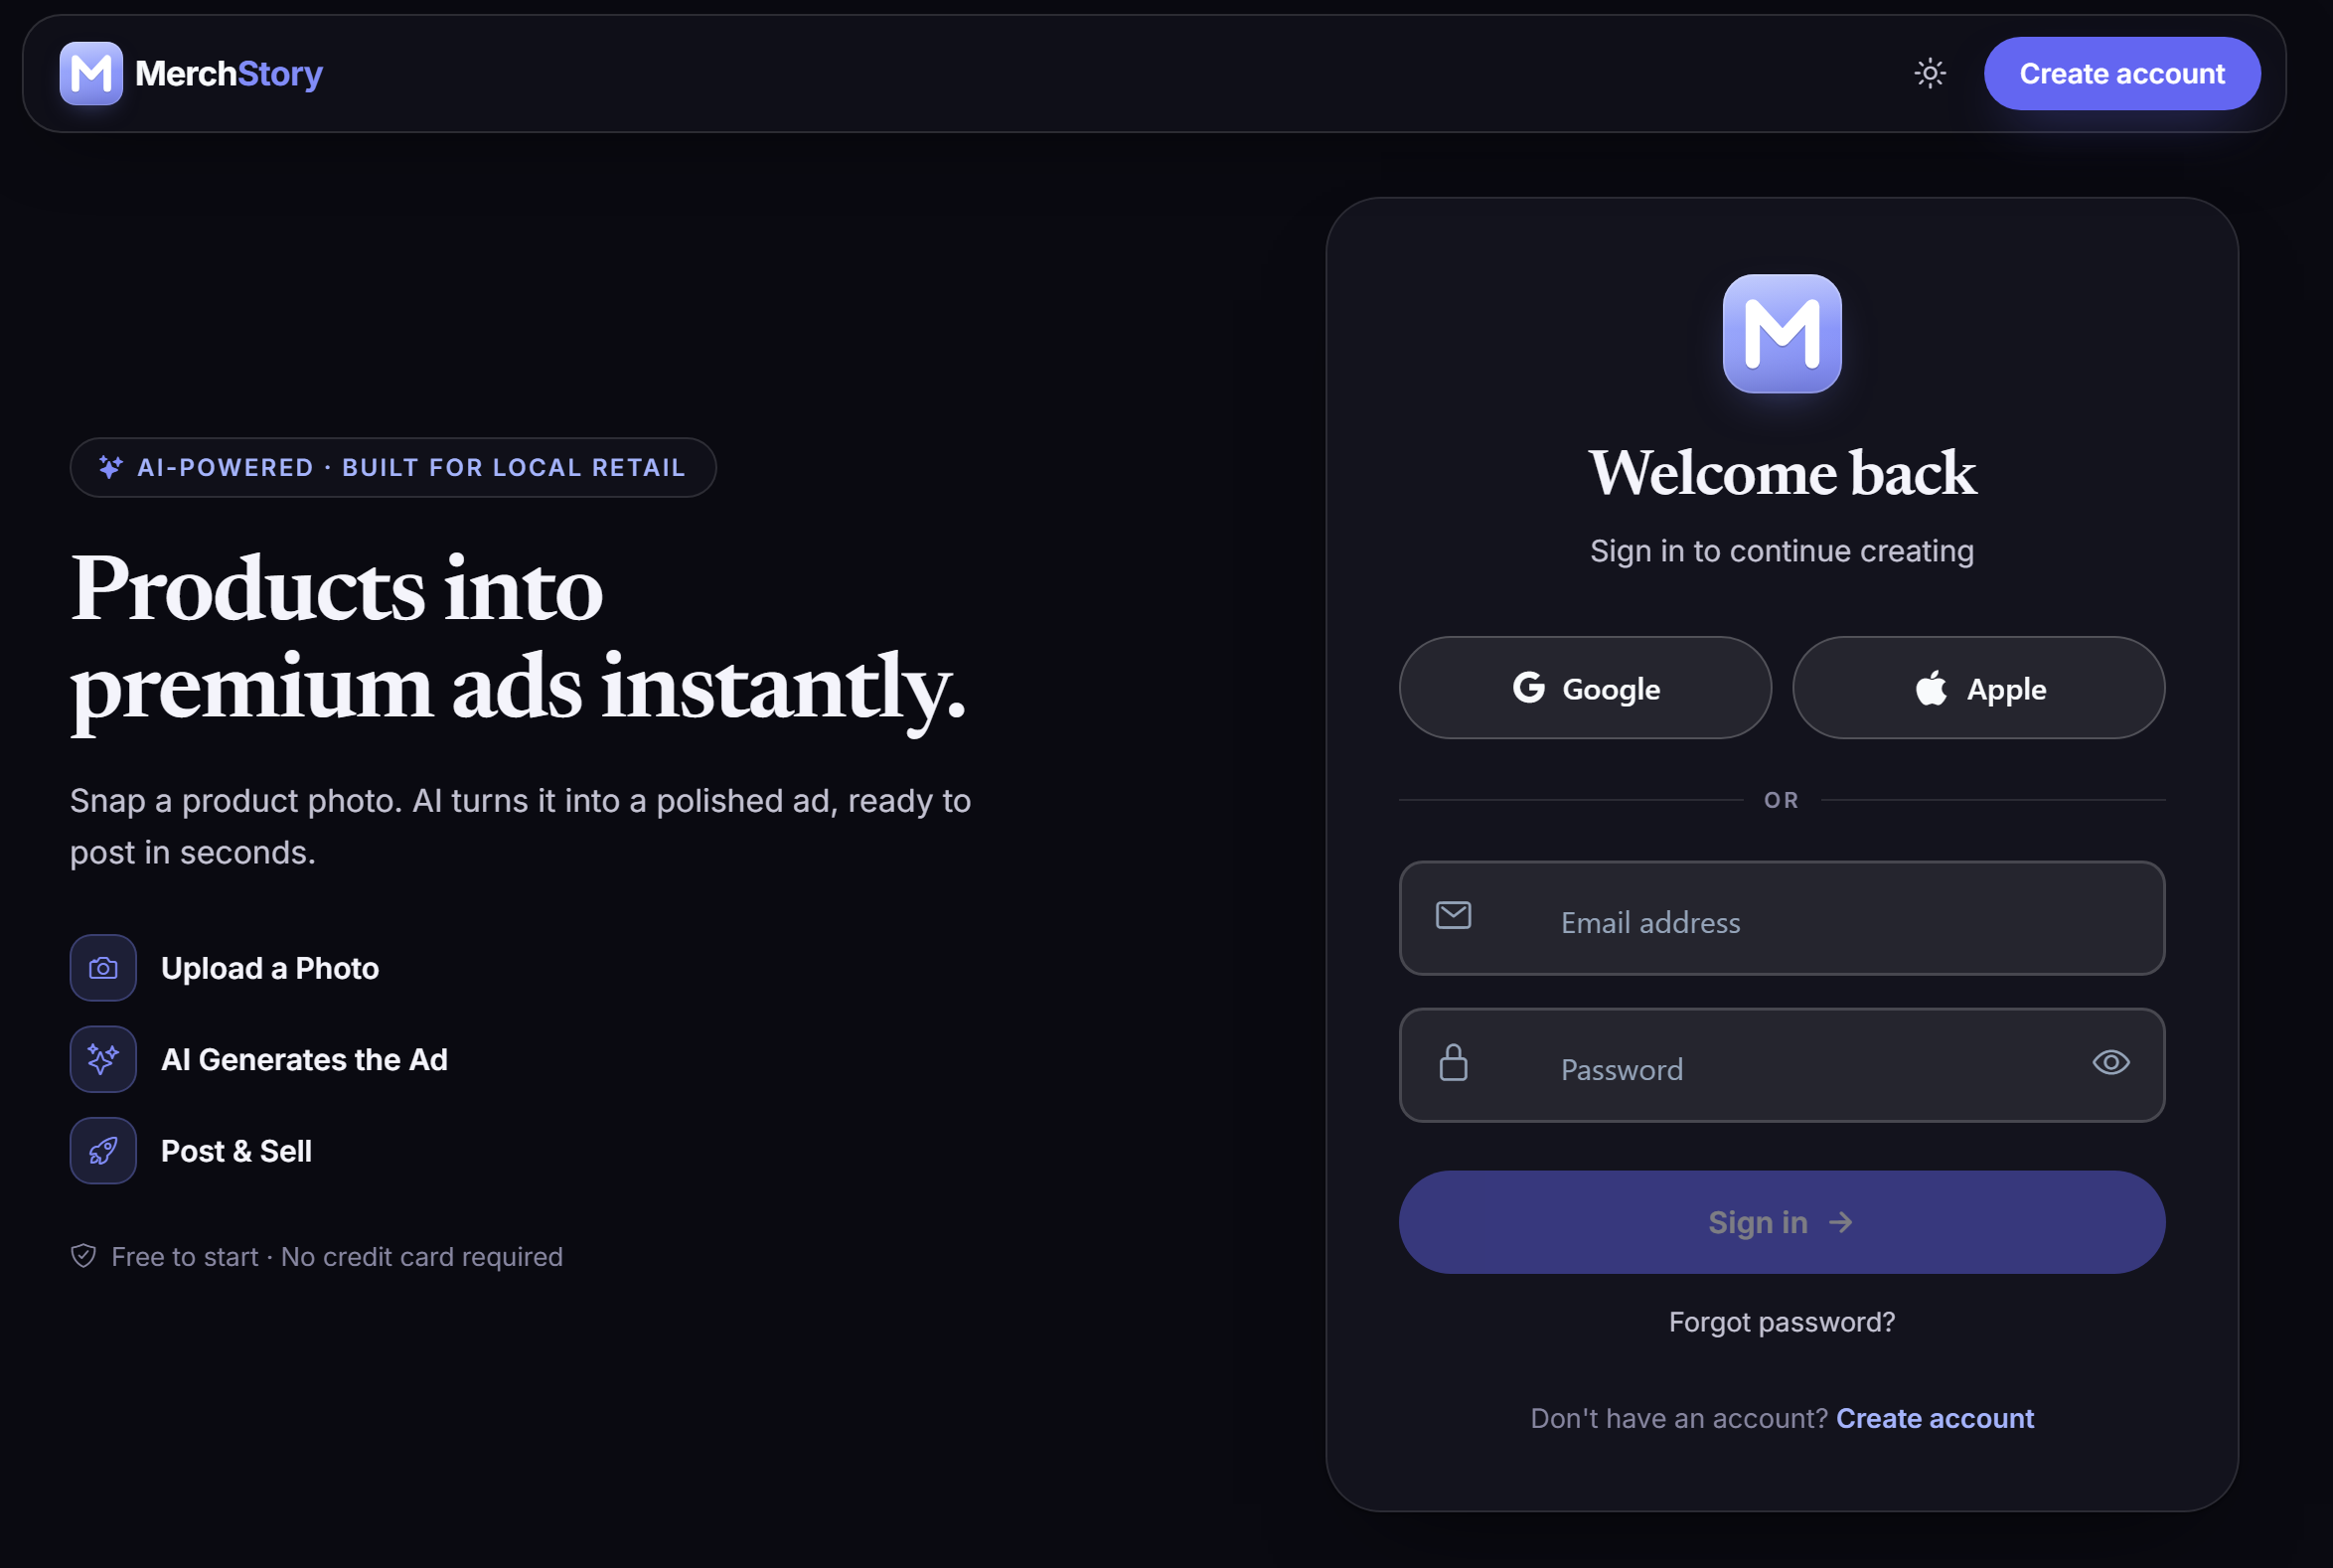
\includegraphics[height=0.28\textwidth]{figures/client/login.png}\hfill
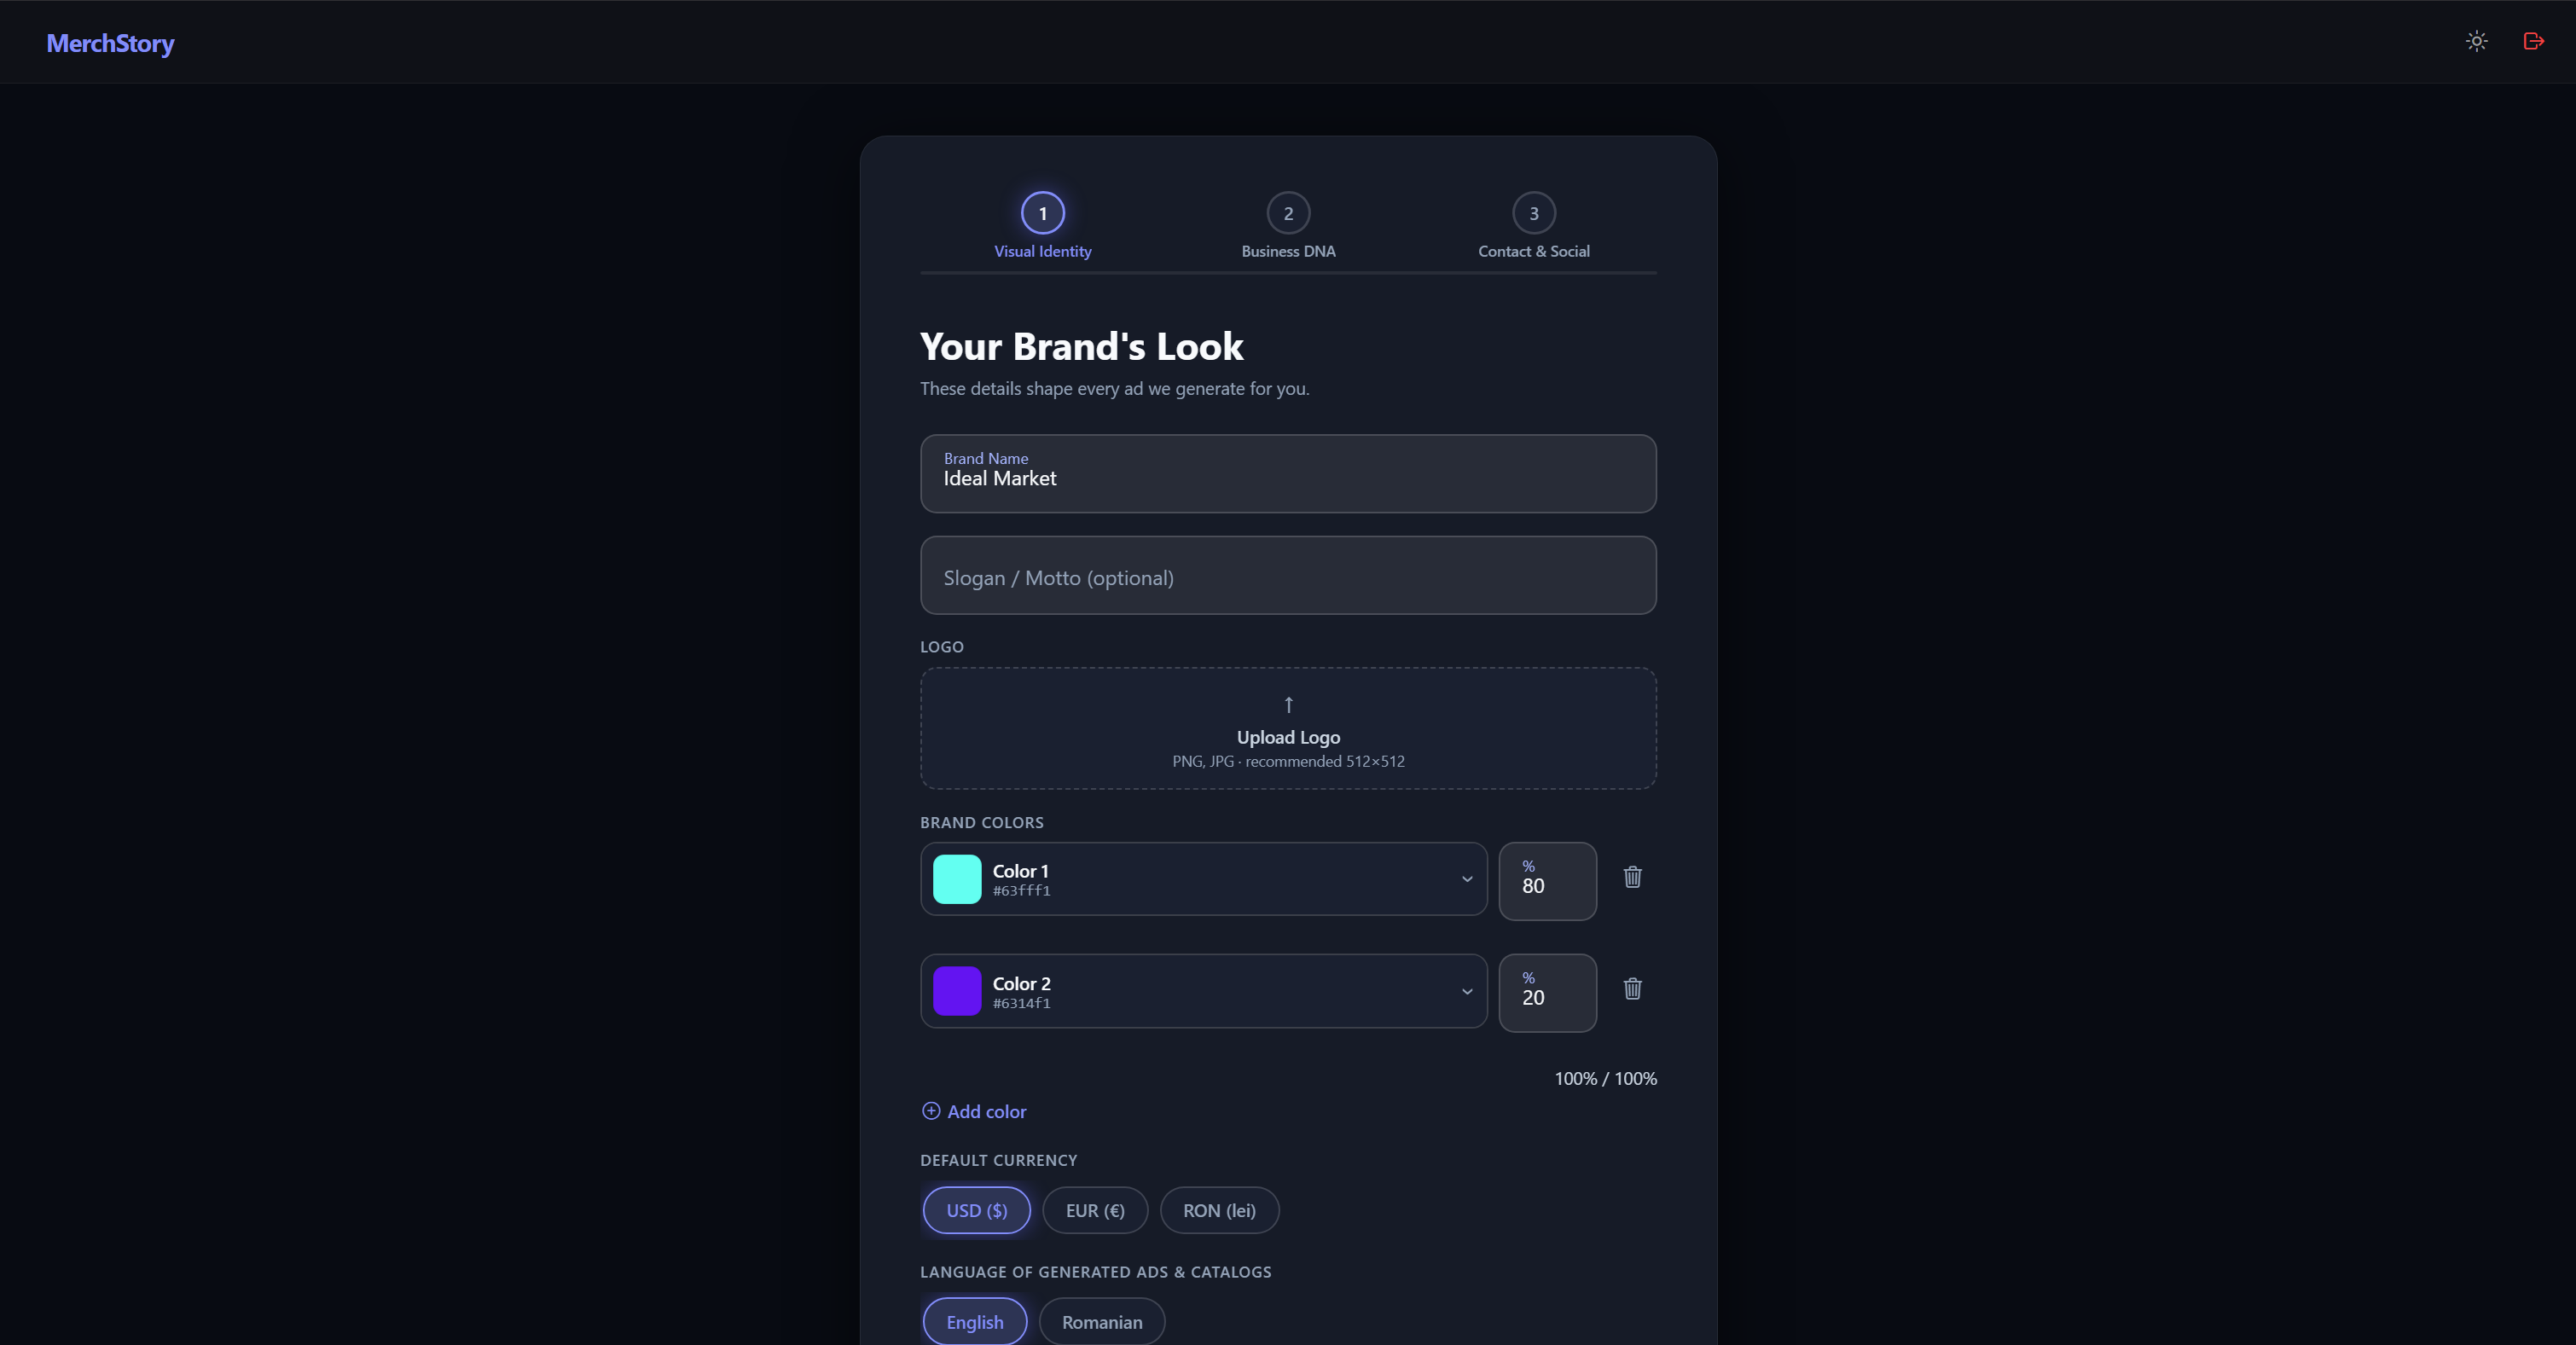
\includegraphics[height=0.28\textwidth]{figures/client/onboarding.png}
\caption{Login screen and shop onboarding step.}
\label{fig:client-auth}
\end{figure}

Once onboarding is complete, the retailer lands on the home surface, a tab bar that gives one-tap access to the main parts of the application. Asset creation is the heart of the daily workflow: the retailer chooses an asset family, picks the products to feature and the model to use, and is shown an explicit progress indicator while the generation runs in the background.

\begin{figure}[!ht]
\centering
\begin{minipage}[t]{0.48\textwidth}
\centering
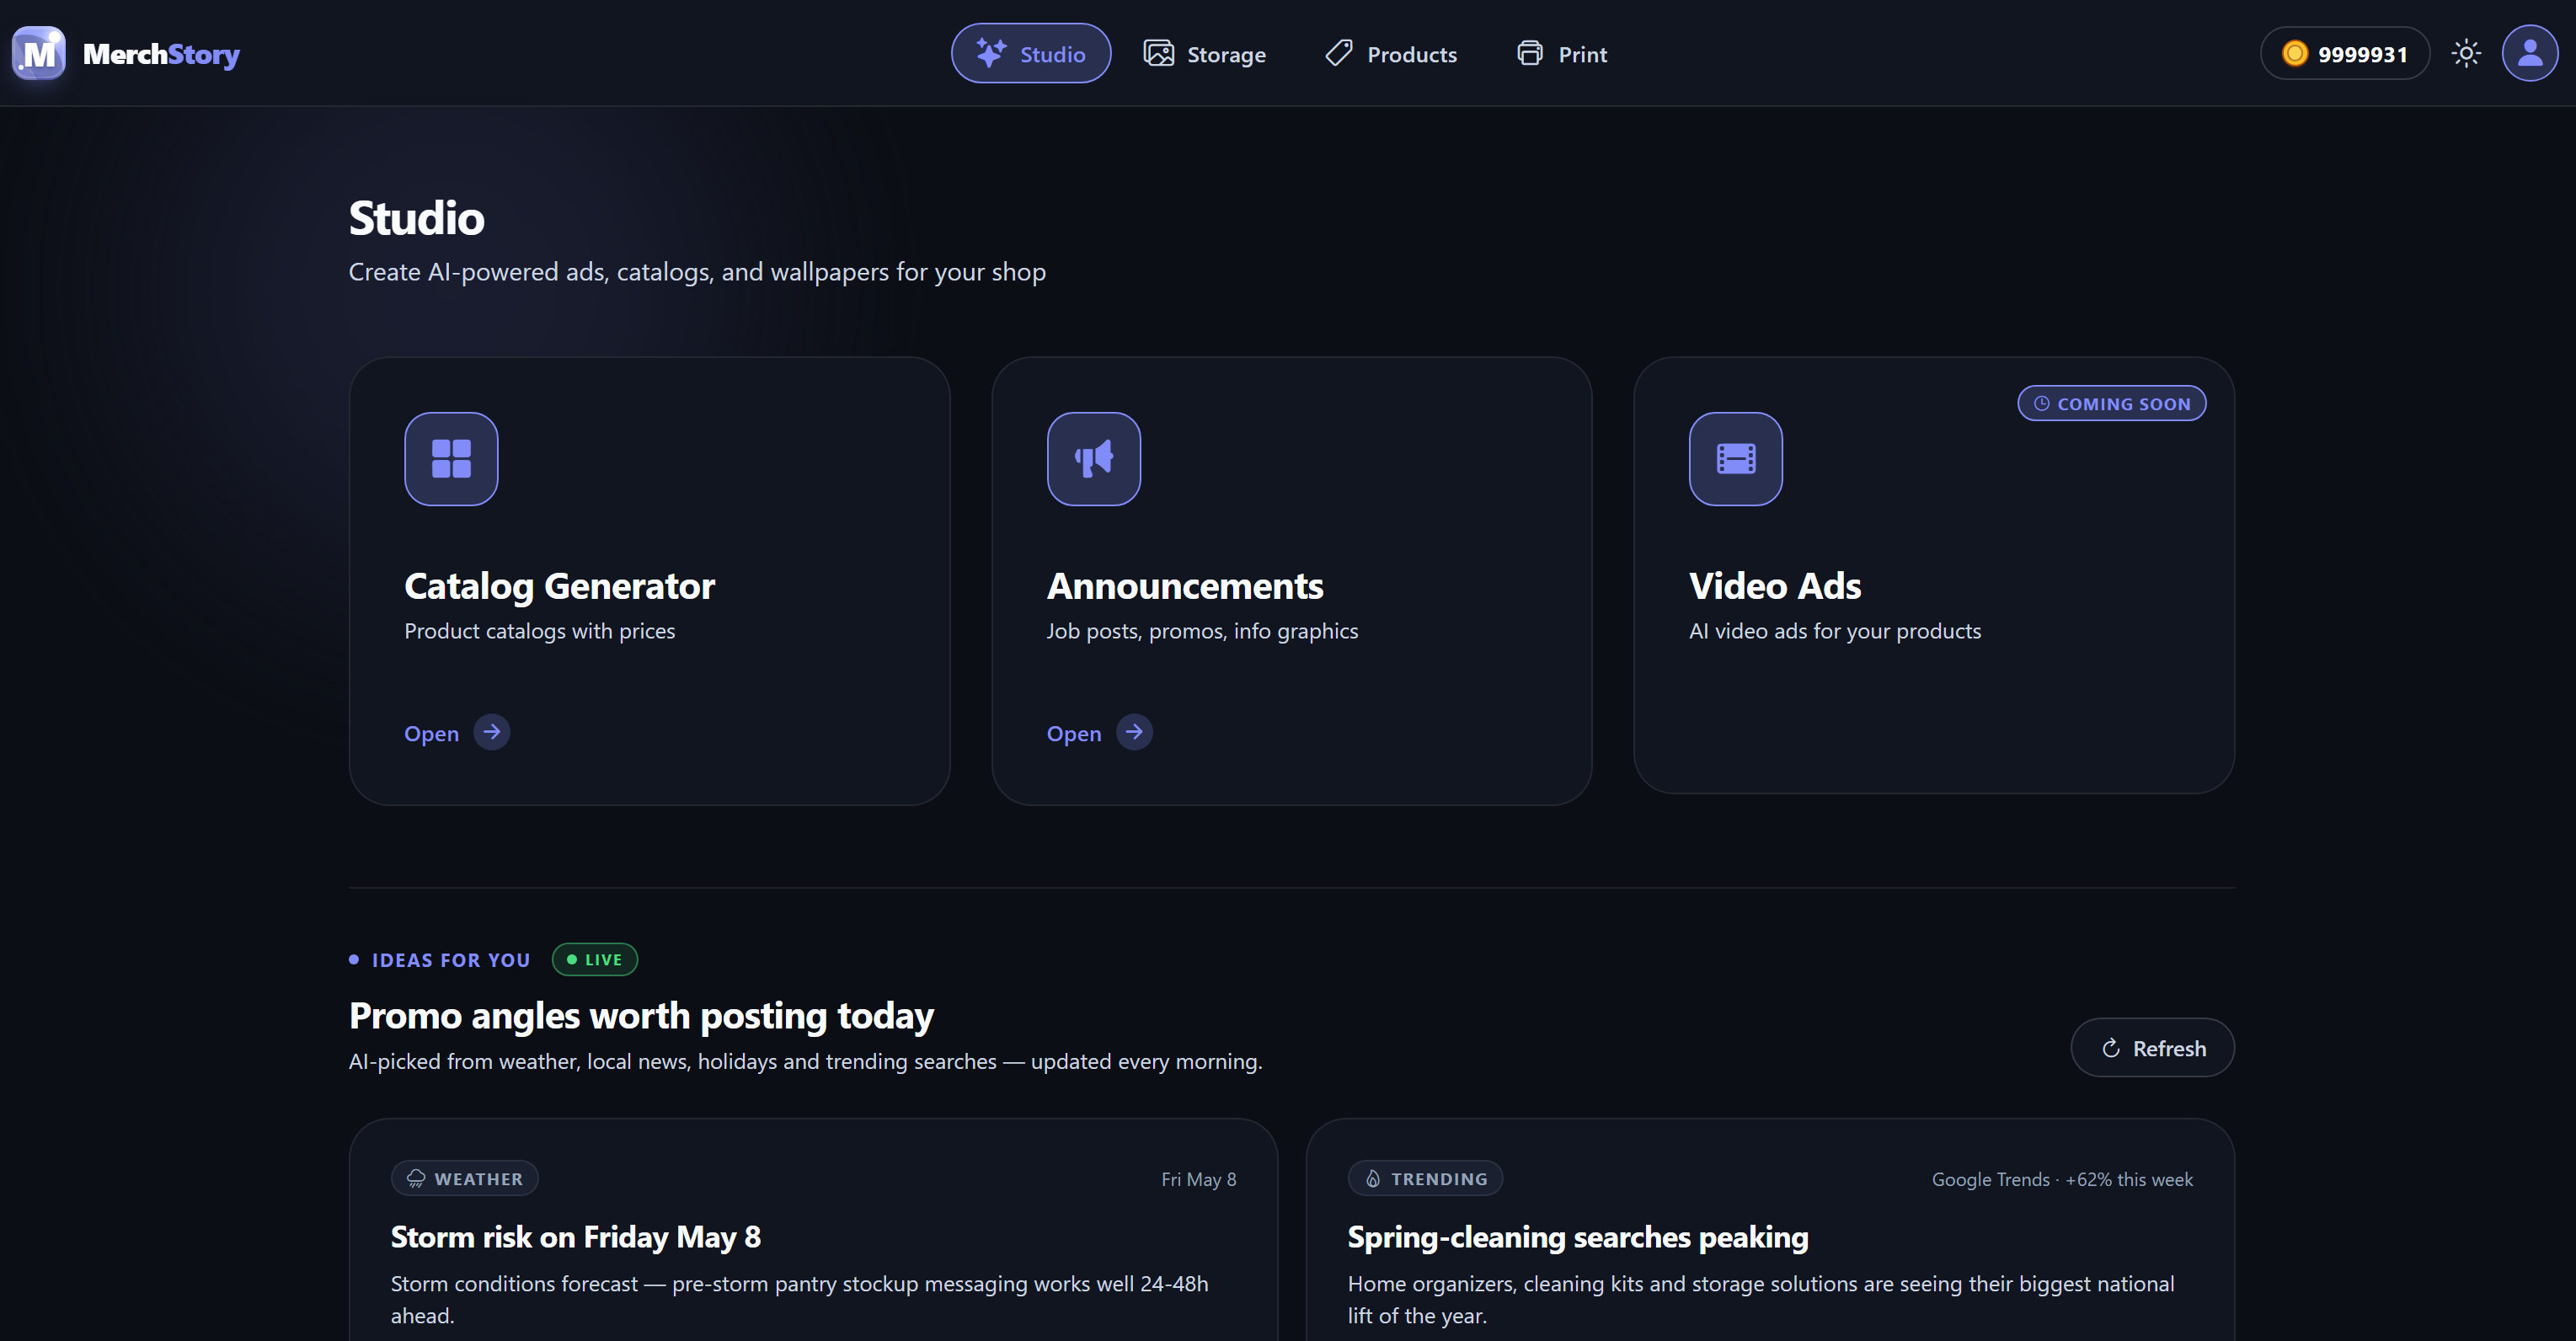
\includegraphics[width=\linewidth]{figures/client/home.png}
\end{minipage}\hfill
\begin{minipage}[t]{0.48\textwidth}
\centering
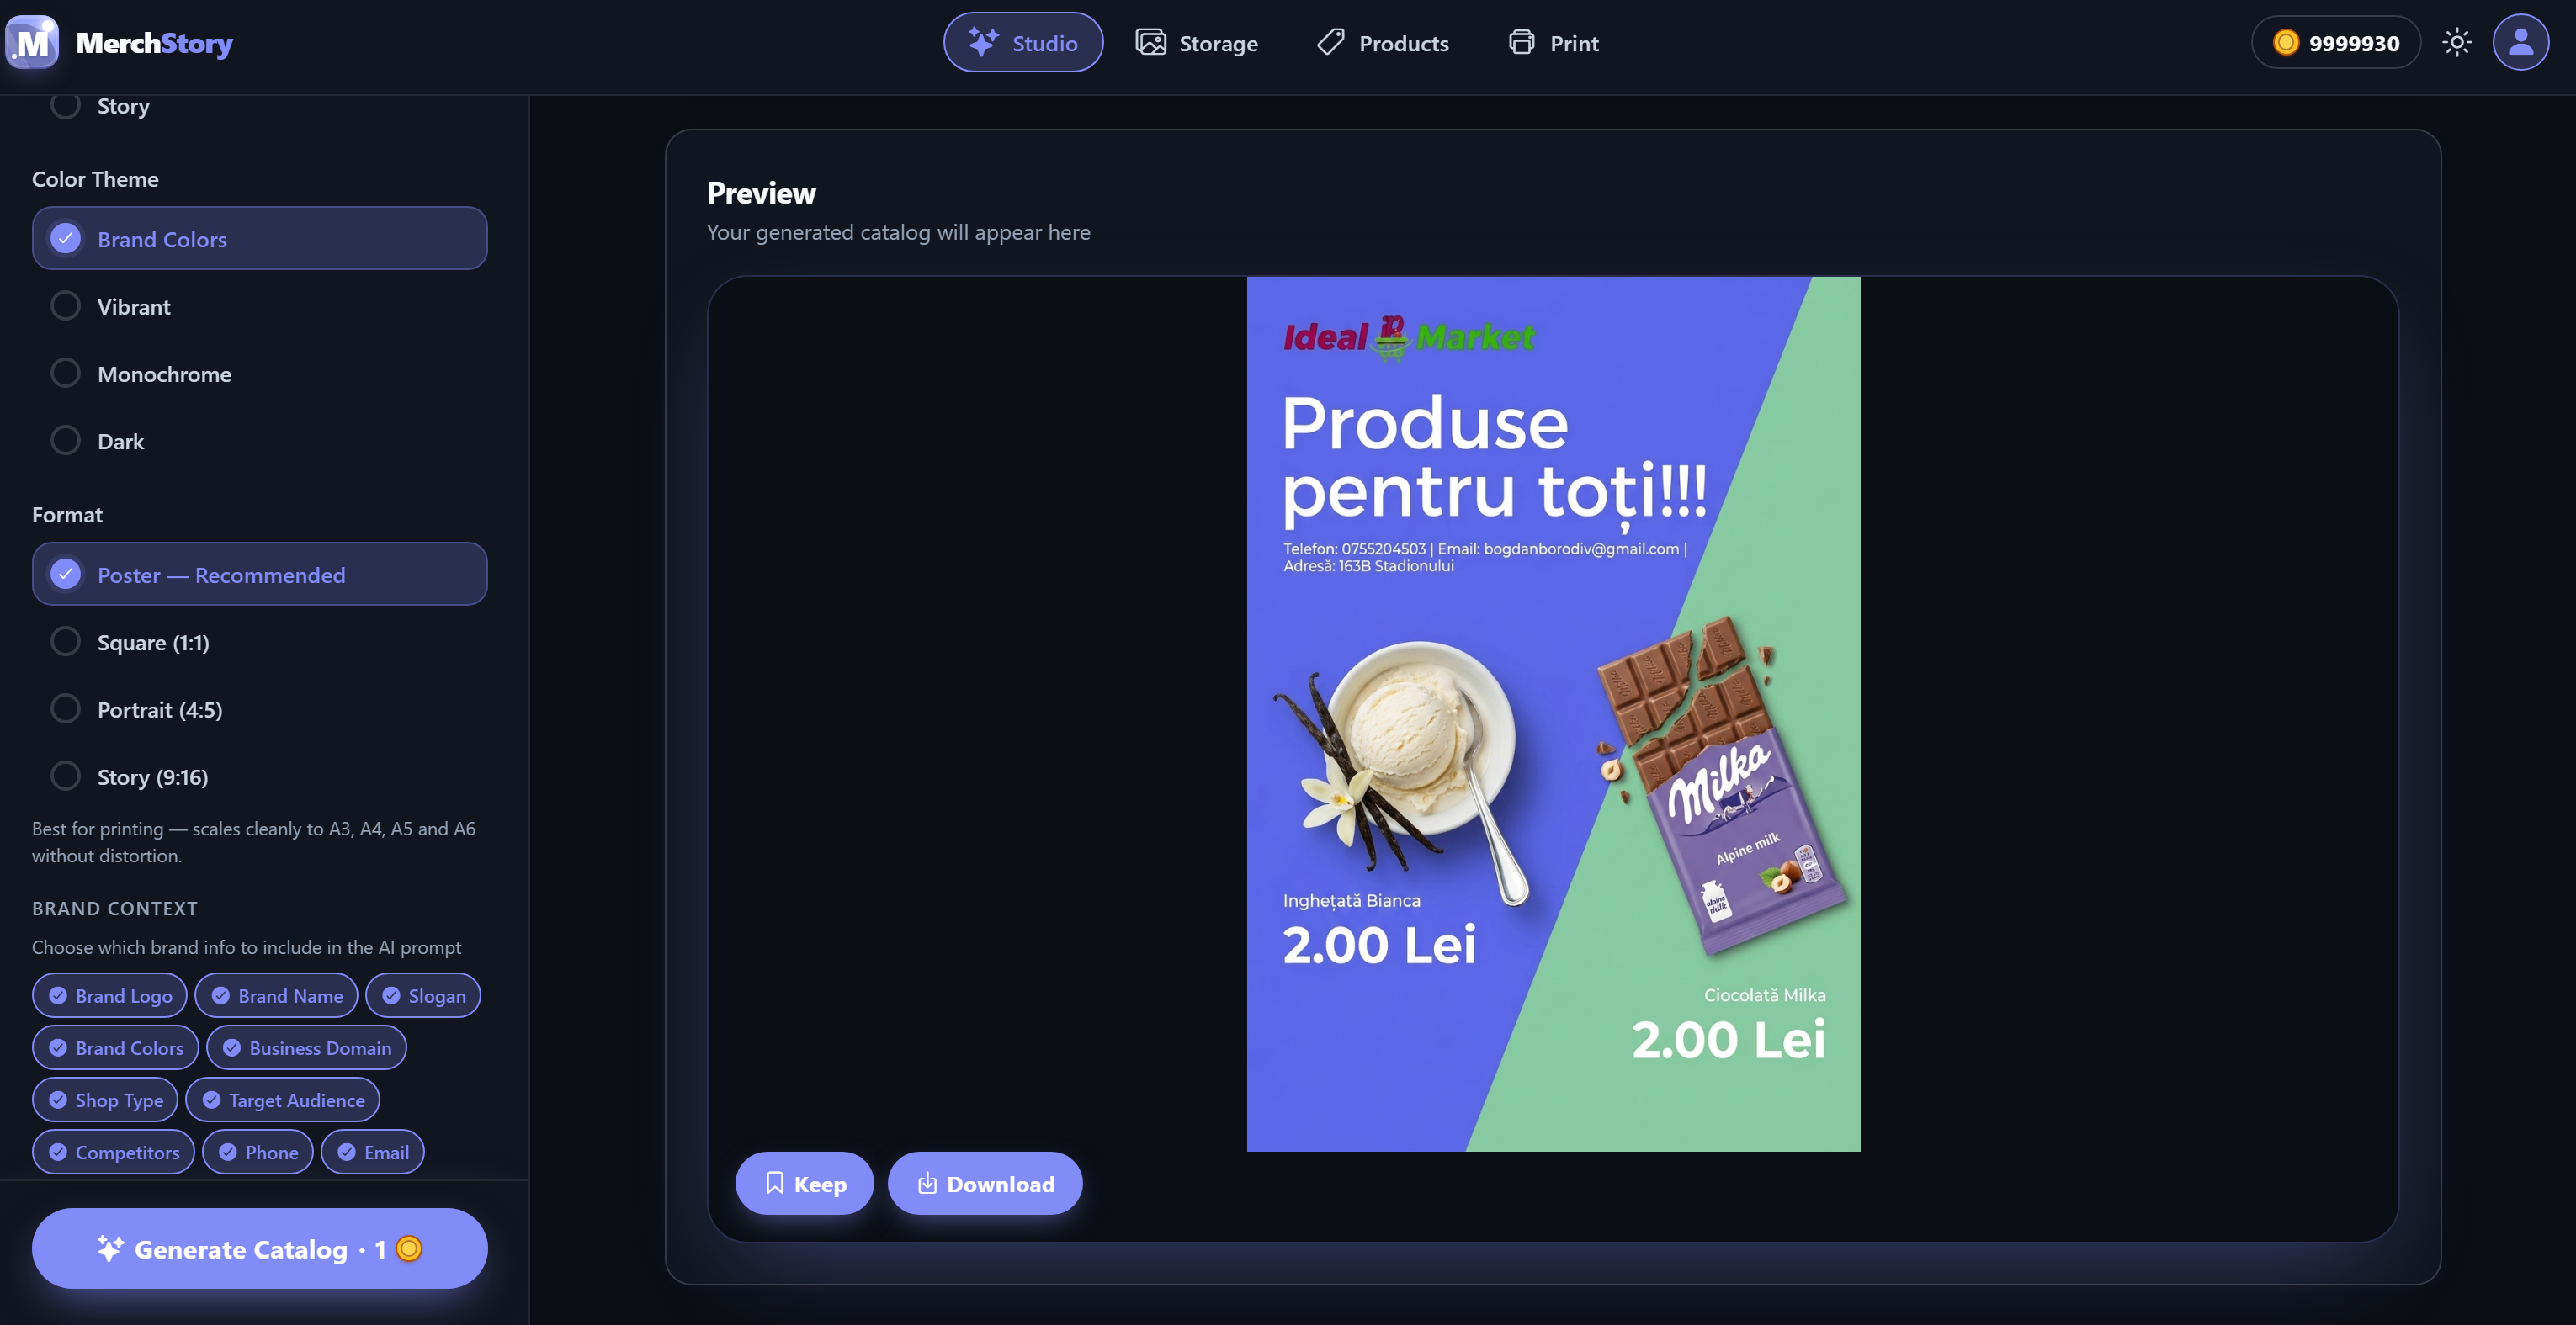
\includegraphics[width=\linewidth]{figures/client/asset-creation.png}
\end{minipage}
\caption{Home tabs and the asset-creation flow.}
\label{fig:client-main}
\end{figure}

Every generated asset is collected in the gallery, where the retailer can browse, filter and export past work. The wallet shows the credit balance and the history of debits and refunds, so the cost of each generation is visible and auditable from the same tab bar.

\begin{figure}[!ht]
\centering
\begin{minipage}[t]{0.48\textwidth}
\centering
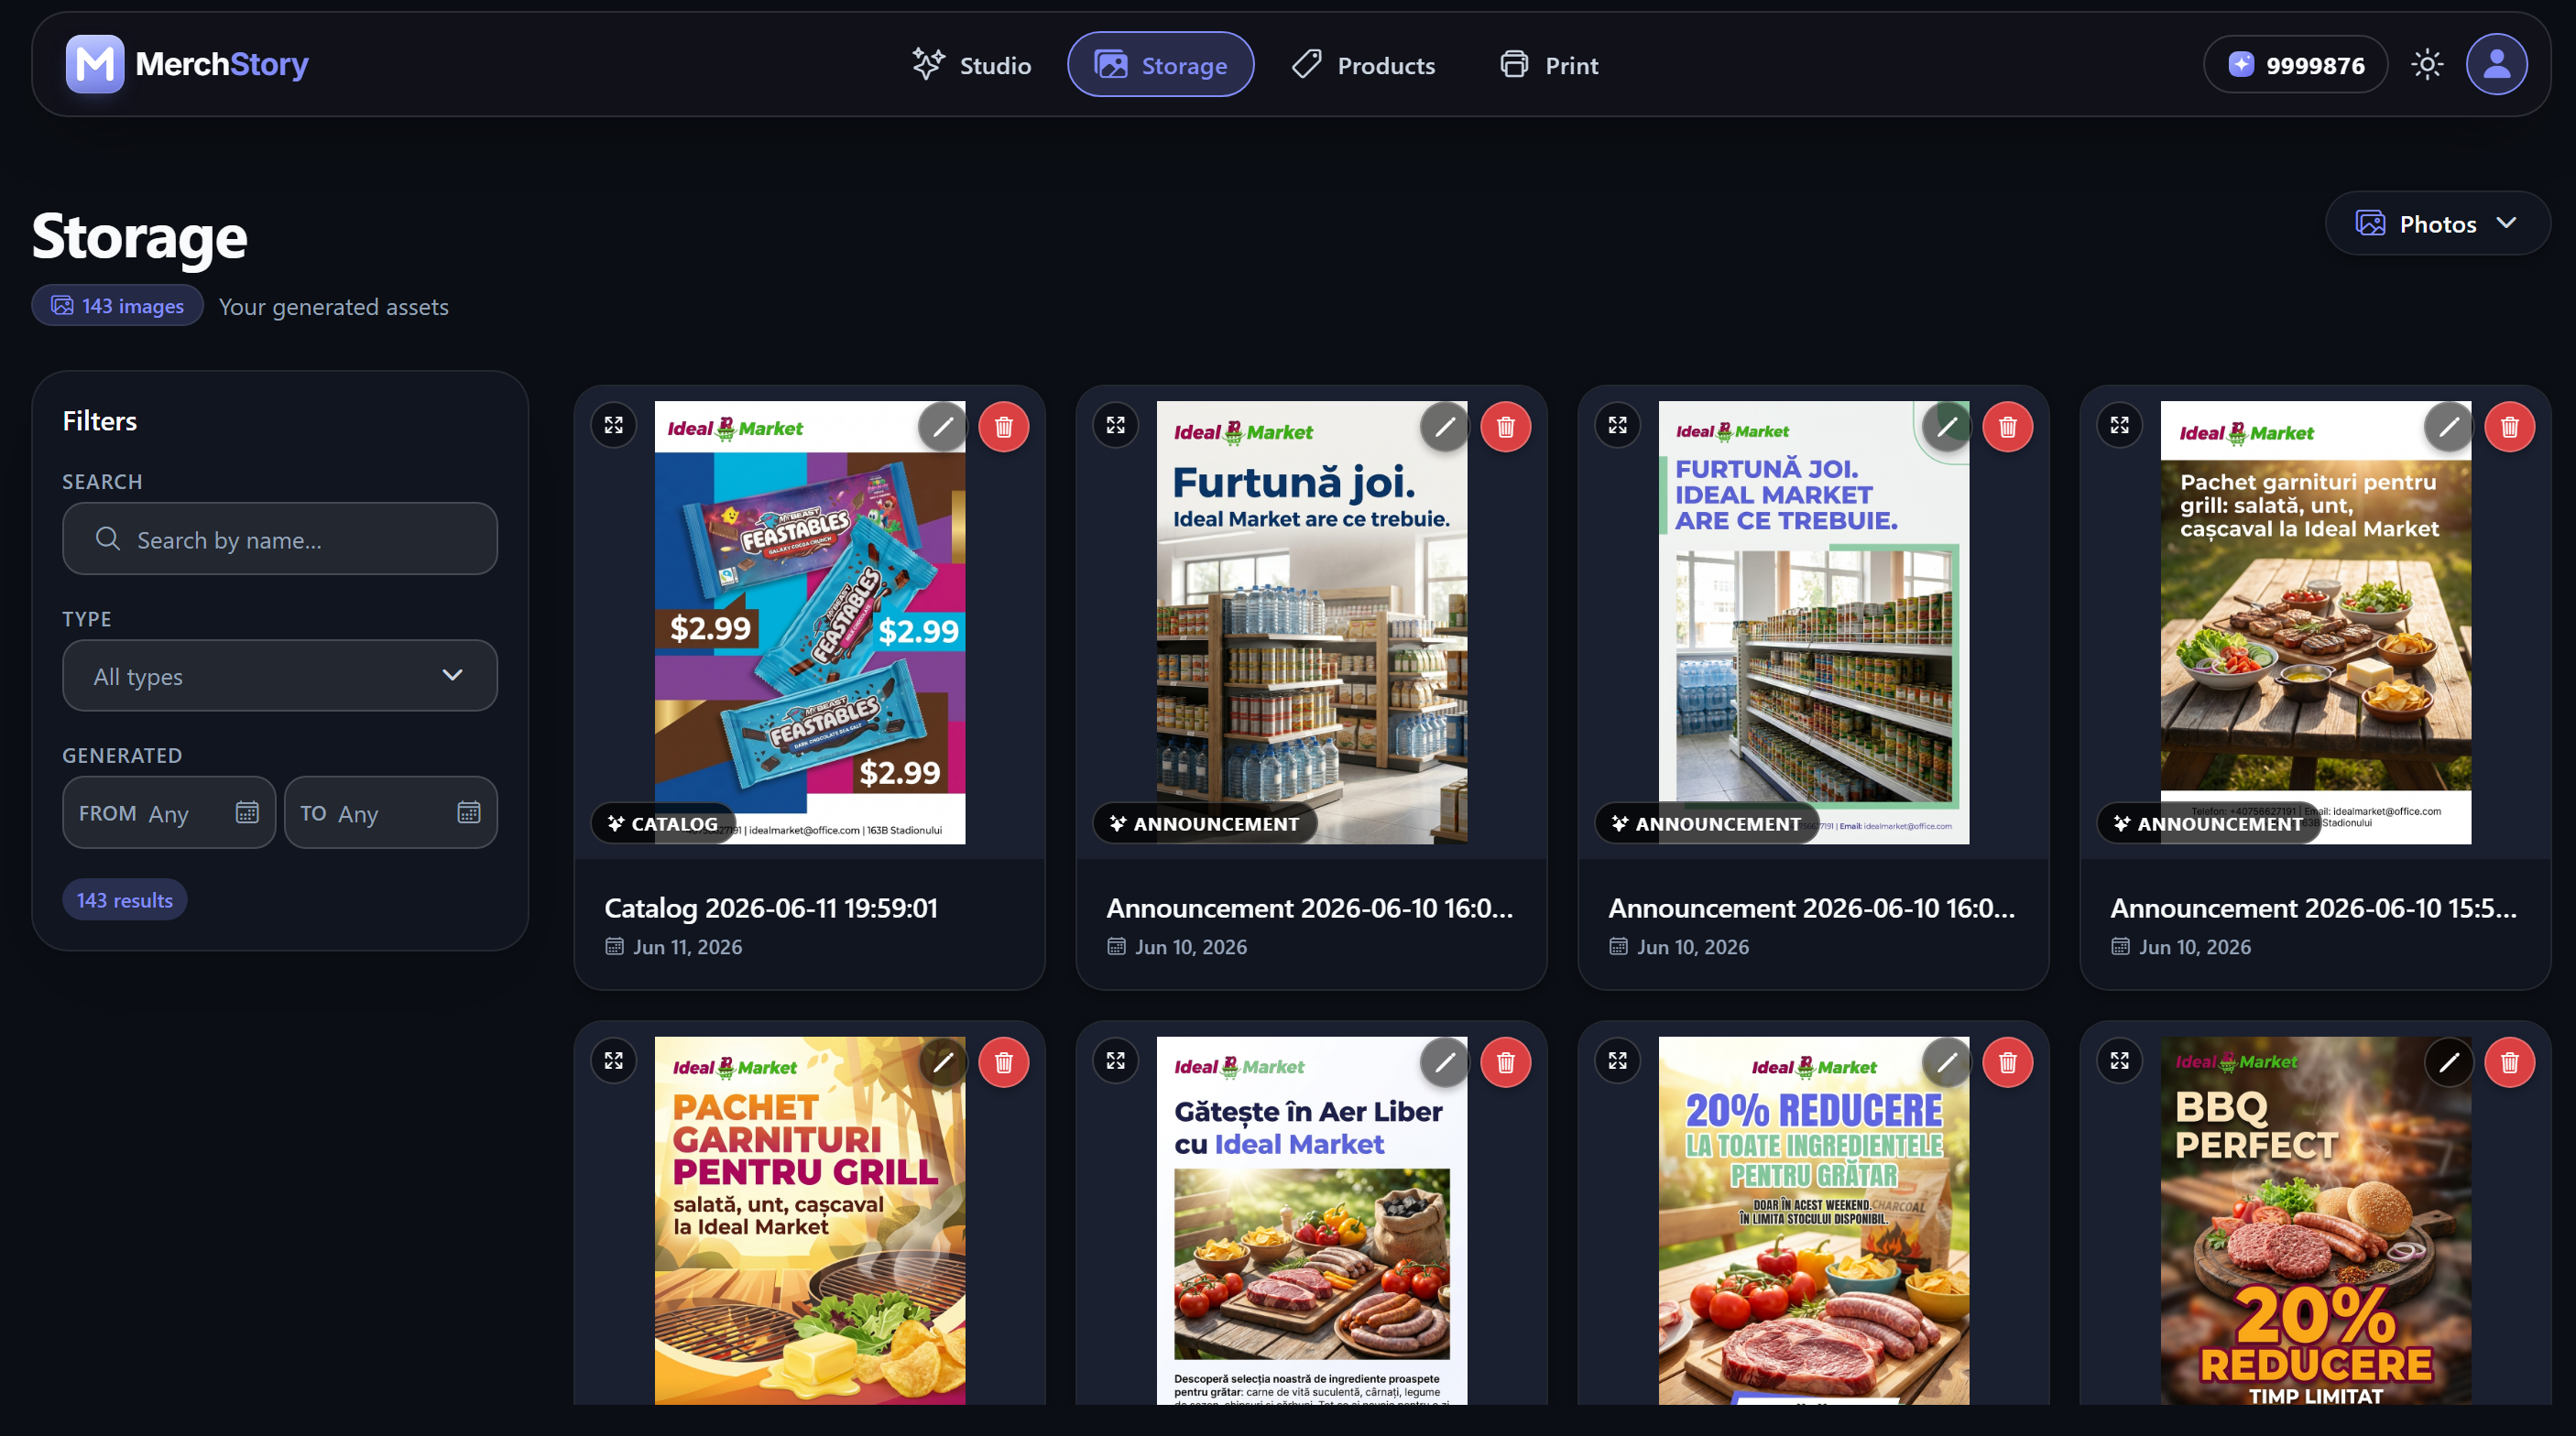
\includegraphics[width=\linewidth]{figures/client/gallery.png}
\end{minipage}\hfill
\begin{minipage}[t]{0.48\textwidth}
\centering
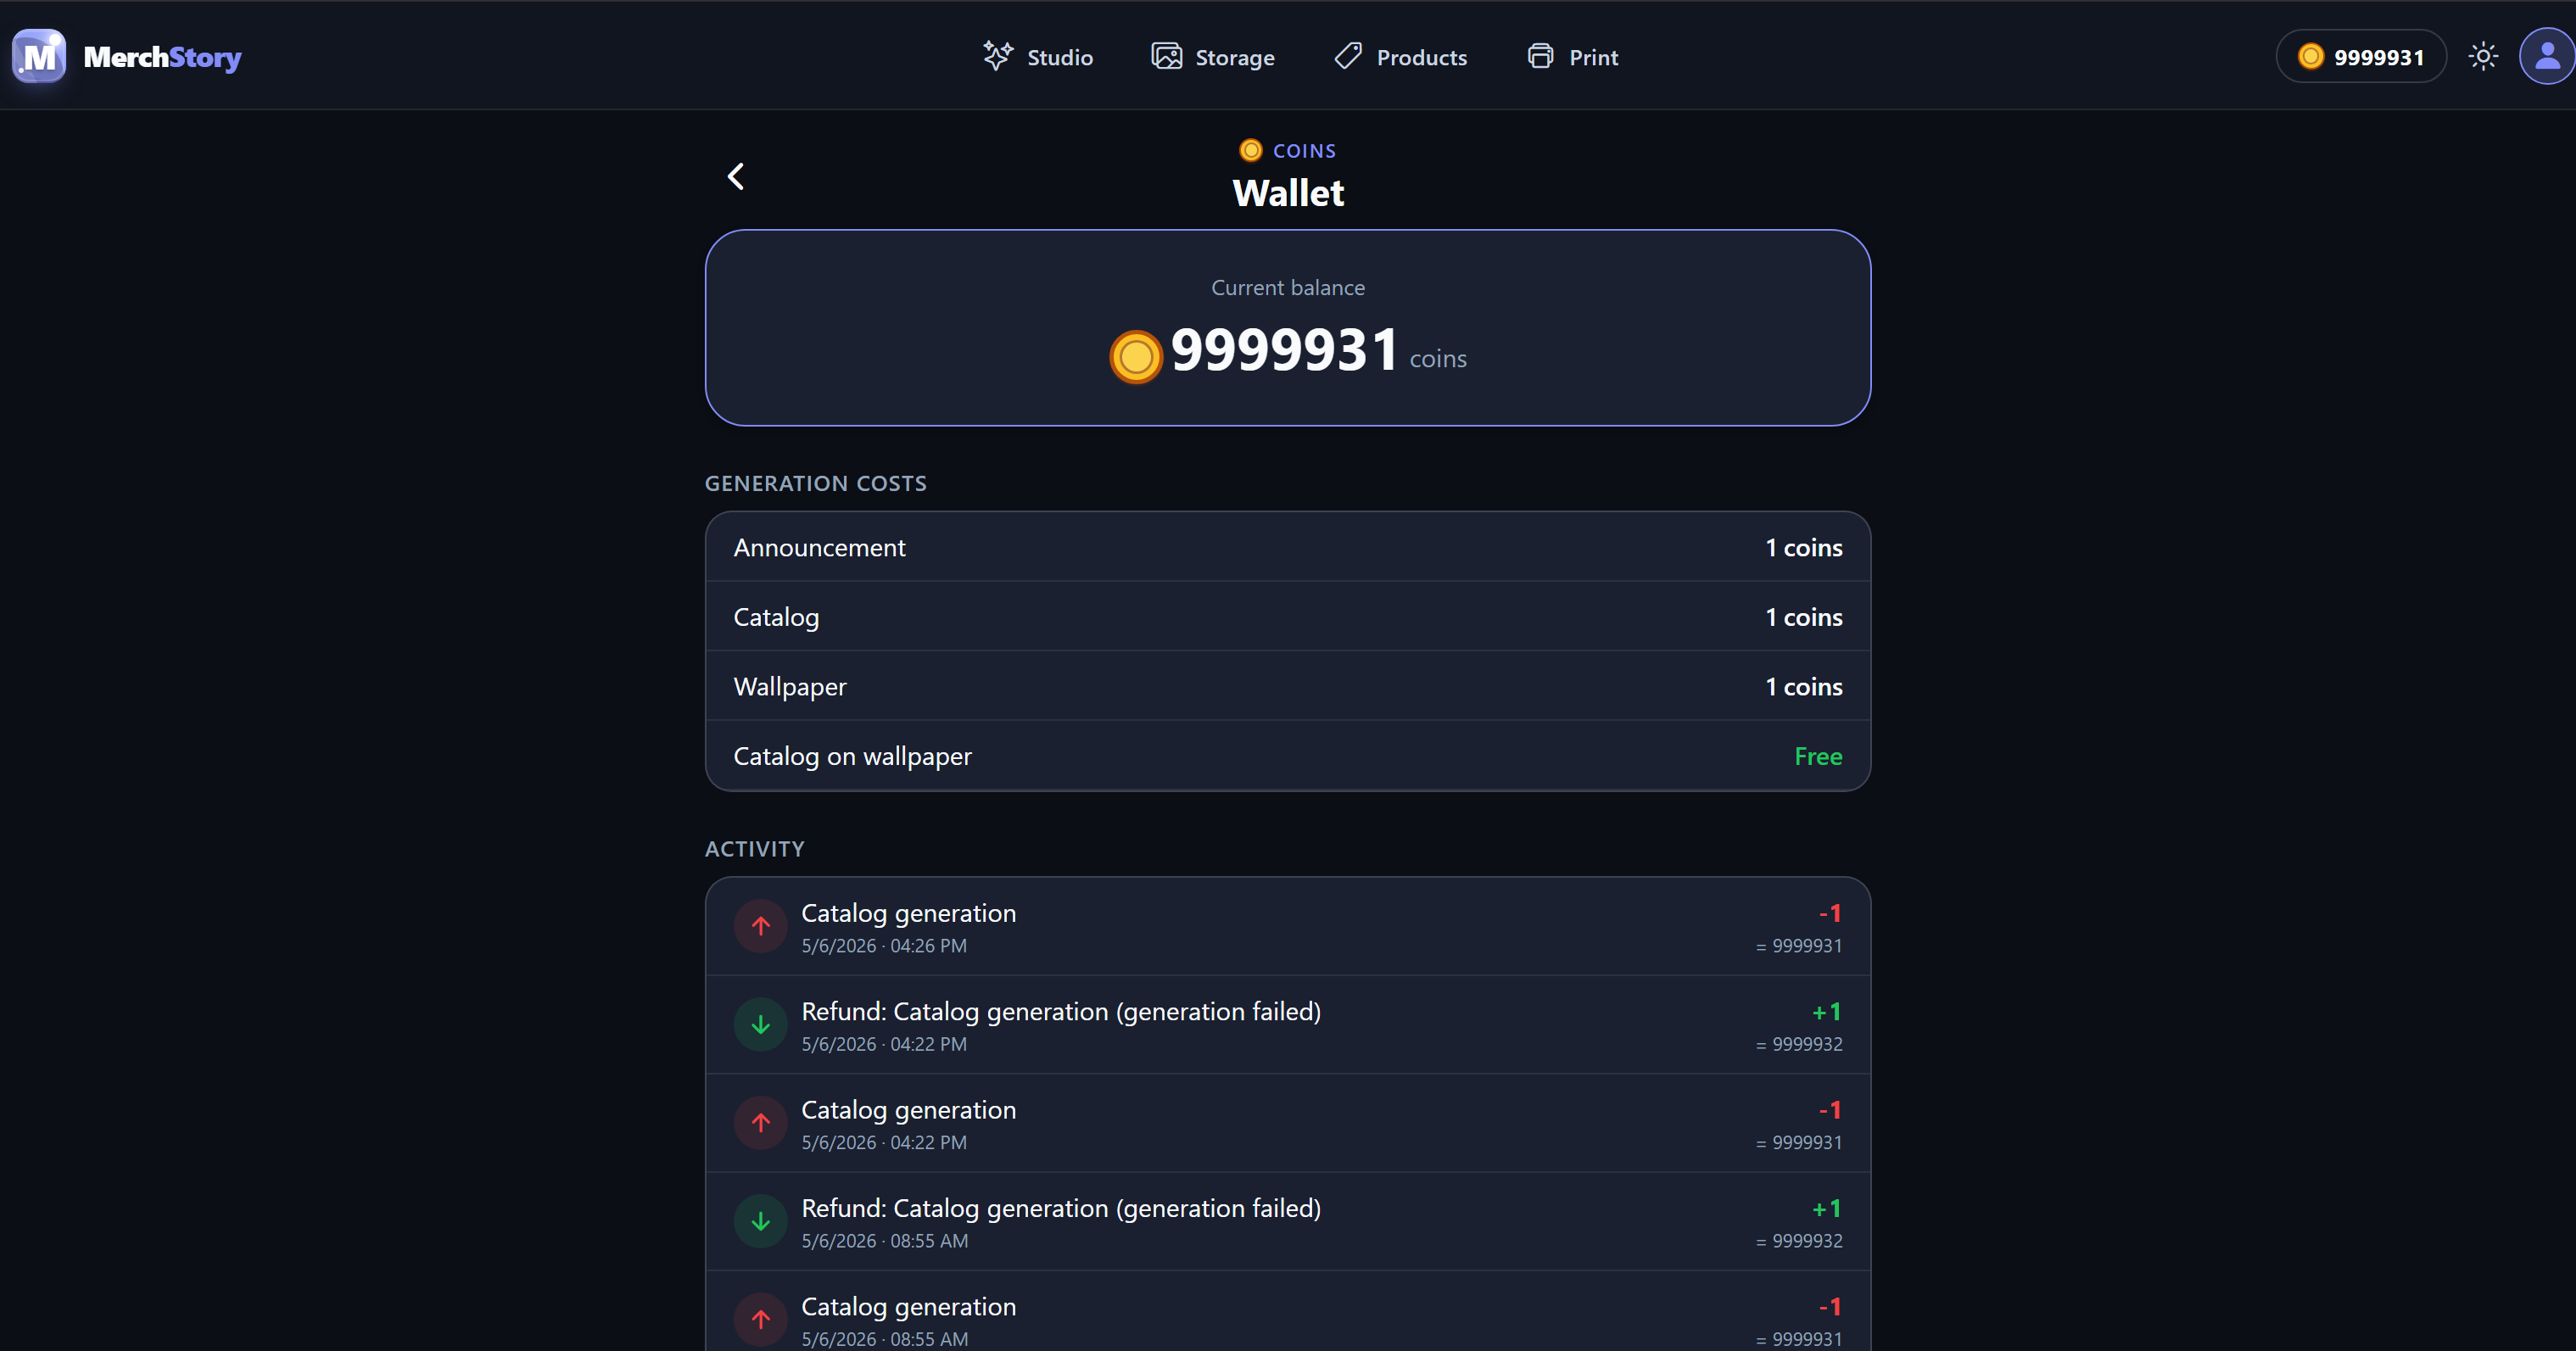
\includegraphics[width=\linewidth]{figures/client/wallet.png}
\end{minipage}
\caption{Gallery and wallet screens.}
\label{fig:client-output}
\end{figure}

\section{Application Server}
\label{sec:application-server}

The application server is a minimal-API ASP.NET Core service running on .NET 10. It hosts every feature service the platform exposes. It also hosts the two provider abstractions that AI calls pass through before they leave the server. Semantic Kernel handles the language-model work, and \textbf{IImageProvider} handles image generation.

\subsection{Stack choice, capability areas and internal layering}
\label{subsec:why-dotnet}

The choice of platform deserves comment because .NET is a less obvious pick for a contemporary AI application than Node.js or Python. One important part of the platform is a layer that orchestrates language-model calls. It routes prompts to several model backends, manages prompt templates, adds retrieval-augmented context to those calls, and runs several calls in a row for the daily recommendation engine. Microsoft's \emph{Semantic Kernel} \cite{semantickernel} is a first-class .NET library that bundles all of these facilities behind a unified abstraction, with clean integration into the ASP.NET Core dependency-injection container. Building the server in .NET therefore makes Semantic Kernel a native citizen of the architecture rather than a foreign component, which is the decisive reason for choosing ASP.NET Core minimal-API over Node.js with Express or Python with FastAPI.

Choosing Semantic Kernel does not tie the platform to one model vendor. The recommendation pipeline can run on local open-weight models through LM Studio or Ollama, on hosted DeepSeek or on OpenAI, and switching between them is a configuration change. Image generation does not use Semantic Kernel at all. It sits behind a separate interface called \textbf{IImageProvider}. In production this interface calls Google's Gemini image model, and it can also call OpenAI's GPT Image 2 model through the same interface. The image model can be changed from inside the platform, with no code change. Figure~\ref{fig:semantic-kernel} shows this arrangement.

\begin{figure}[!ht]
\centering
% --- same palette as Figure \ref{fig:three-tier} ---
\definecolor{cInk}{HTML}{2E3440}    % text + arrows
\definecolor{cIndigo}{HTML}{3F4D8C} % abstraction layers
\definecolor{cSlate}{HTML}{4A5568}  % application server
\definecolor{cGray}{HTML}{7C8390}   % backends
\resizebox{\textwidth}{!}{%
\begin{tikzpicture}[
    font=\sffamily\scriptsize,
    bar/.style={draw=#1, line width=0.9pt, rounded corners=3pt, align=center,
                text=cInk, drop shadow={shadow xshift=0.5mm, shadow yshift=-0.5mm,
                                        fill=black, opacity=0.12}},
    groupcard/.style={draw=#1, line width=0.9pt, rounded corners=3pt, inner sep=0pt,
                      dash pattern=on 2.4pt off 1.7pt, fill=#1!6},
    tab/.style={fill=#1, rounded corners=2.5pt, inner xsep=6pt, inner ysep=0pt,
                minimum height=5.2mm, anchor=south west,
                font=\sffamily\scriptsize\bfseries, text=white},
    chip/.style={draw=#1, line width=0.6pt, rounded corners=2.5pt, fill=white,
                 minimum height=9mm, align=center, text=cInk},
    arr/.style={-{Latex[length=2mm,width=1.5mm]}, line width=0.7pt, draw=cInk!85}
]

% ============ application server (top, full width) ============
\node[bar=cSlate, fill=cSlate!8, minimum width=150mm, minimum height=10mm]
      (api) at (0,5.0) {\textbf{Application server} \quad (ASP.NET Core, .NET 10)};

% ============ abstraction bars ============
\node[bar=cIndigo, fill=cIndigo!14, minimum width=84mm, minimum height=13mm]
      (sk) at (-3.3,3.0)
      {\textbf{Semantic Kernel}\\prompt templates \;$\cdot$\; retrieval-augmented context \;$\cdot$\; multi-stage chaining};
\node[bar=cIndigo, fill=cIndigo!14, minimum width=56mm, minimum height=13mm]
      (iface) at (4.5,3.0)
      {\textbf{IImageProvider}\\image generation};

% ============ backend group cards ============
\node[groupcard=cGray, minimum width=84mm, minimum height=28.5mm] (llmCard) at (-3.3,-0.03) {};
\node[groupcard=cGray, minimum width=56mm, minimum height=28.5mm] (imgCard) at ( 4.5,-0.03) {};

% ============ language-model backend chips ============
\node[chip=cGray, minimum width=38mm] (loc) at (-5.4, 0.65) {Local\\(LM Studio / Ollama)};
\node[chip=cGray, minimum width=28mm] (ds)  at (-1.7, 0.65) {DeepSeek};
\node[chip=cGray, minimum width=28mm] (oa)  at (-3.55,-0.70) {OpenAI};

% ============ image-generation backend chips ============
\node[chip=cGray, minimum width=50mm] (gem) at (4.5, 0.65) {Google Gemini};
\node[chip=cGray, minimum width=50mm] (gpt) at (4.5,-0.70) {GPT Image 2};

% ============ arrows ============
\draw[arr] (api.south) -- (sk.north);
\draw[arr] (api.south) -- (iface.north);
\draw[arr] (sk.south)    -- (llmCard.north);
\draw[arr] (iface.south) -- (imgCard.north);

% ============ group tabs (drawn last so they sit above the arrows) ============
\node[tab=cIndigo] at ([xshift=4mm]llmCard.north west) {Language-model backends};
\node[tab=cIndigo] at ([xshift=4mm]imgCard.north west) {Image-generation backends};

\end{tikzpicture}%
}
\caption{Provider abstractions on the application server.}
\label{fig:semantic-kernel}
\end{figure}

\label{subsec:capabilities}
Each capability area on the server is a bounded service that exposes a small set of HTTP endpoints. Authentication is handled inside the server itself: a successful login produces a short-lived JWT access token and a longer-lived refresh token. The access token is validated locally on every request, the refresh token is stored in the database and is rotated each time it is used, and a background service periodically removes tokens that have expired or been revoked.

The retailer-facing entities (shop profile, products, gallery, wallet) are each served by a dedicated feature service that exposes CRUD operations over its part of the schema, with the isolation rules inherited from the data layer. Coordination between services is performed at the endpoint layer rather than through direct inter-service calls.

A thin orchestration layer fronts the supported image providers behind a single \textbf{IImageProvider} abstraction shown in Listing~\ref{lst:iimageprovider}. Each provider has a concrete implementation that wraps its SDK, and a mock implementation returns a deterministic placeholder image during automated testing.

\begin{lstlisting}[style=csharp, caption={The IImageProvider abstraction.}, label={lst:iimageprovider}]
public interface IImageProvider
{
    Task<ImageGenerationResult> GenerateAsync(
        string prompt,
        IReadOnlyList<string?>? inlineImages = null,
        CancellationToken cancellationToken = default);
}
\end{lstlisting}

The daily recommendation engine is exposed as its own service, whose inputs and outputs match the functional requirement above and whose internals are the subject of the contributions chapter that follows. Sitting alongside it is the credit ledger, an in-process service that mediates between every billable AI call and the database. The ledger exposes a single primitive, \emph{run-with-debit}, which opens a database transaction, debits the cost, runs the work, and commits only when the work succeeds. A failure rolls the transaction back so that no debit is ever recorded for unsuccessful work.

Two long-running background services run in the same process as the request handler: a job runner that consumes pending recommendation runs, and a cleaner that deletes expired refresh tokens. At the platform's data volumes a separate worker tier is not justified. All of this is exposed over a small, feature-grouped HTTP API; Table~\ref{tab:http-endpoints} lists each route group along with its prefix and purpose.

{\small
\renewcommand{\arraystretch}{1.3}
\begin{tabularx}{\textwidth}{|>{\raggedright\arraybackslash}p{3.2cm}|>{\raggedright\arraybackslash}p{3.6cm}|Y|}
\caption{HTTP route groups exposed by the application server.}\label{tab:http-endpoints}\\
\hline
\textbf{Group} & \textbf{Prefix} & \textbf{Purpose} \\
\hline
\endfirsthead
\hline
\textbf{Group} & \textbf{Prefix} & \textbf{Purpose} \\
\hline
\endhead
\hline
\endfoot
\hline
\endlastfoot
Auth & /auth & Register, log in, refresh tokens and change interface language. \\
\hline
Shop & /shop & Read and update the shop profile and logo. \\
\hline
Products & /products & CRUD over the retailer's product library, with one-tap background removal. \\
\hline
Reference catalogue & /reference-images & Browse, search and bulk-import the curated reference catalogue. \\
\hline
Image generation & /generate-image & Produce announcements, catalogues and wallpapers in fully generative or hybrid mode. \\
\hline
Gallery & /gallery & Save, list, rename and delete generated assets. \\
\hline
Wallet & /wallet & Read the credit balance and ledger, and grant credits (operator only). \\
\hline
Recommendations & /recommendations & Fetch today's ideas, request a refresh and leave feedback. \\
\hline
Print & /print & Render a gallery item to a print-ready document. \\
\end{tabularx}
}

\paragraph{Internal layering.}\label{subsec:server-layering}
Each feature follows a simple internal layering, shown in Figure~\ref{fig:server-layering}. The endpoint layer handles HTTP concerns only and delegates to a feature service that holds the business logic. The feature service then calls the data layer. For AI work it instead calls one of the provider abstractions, which are Semantic Kernel for language-model calls and \textbf{IImageProvider} for image generation. Those abstractions are the only place from which outbound HTTP calls to third parties leave, which keeps retries, circuit breakers and credential management in one place.

\begin{figure}[H]
\centering
% --- same palette as Figure \ref{fig:three-tier} ---
\definecolor{cInk}{HTML}{2E3440}    % text + arrows
\definecolor{cIndigo}{HTML}{3F4D8C} % entry / orchestration
\definecolor{cSlate}{HTML}{4A5568}  % feature internals
\definecolor{cGray}{HTML}{7C8390}   % external boundary
\begin{tikzpicture}[
    font=\sffamily\scriptsize,
    bar/.style={draw=#1, line width=0.9pt, rounded corners=3pt, align=center,
                minimum width=90mm, minimum height=13mm, text=cInk,
                drop shadow={shadow xshift=0.5mm, shadow yshift=-0.5mm,
                             fill=black, opacity=0.12}},
    extbar/.style={draw=cGray, line width=0.9pt, rounded corners=3pt, align=center,
                   dash pattern=on 2.4pt off 1.7pt, fill=cGray!6,
                   minimum width=90mm, minimum height=13mm, text=cInk},
    arr/.style={-{Latex[length=2mm,width=1.5mm]}, line width=0.7pt, draw=cInk!85}
]
\node[bar=cIndigo, fill=cIndigo!7]  (ep)   at (0,0)
      {\textbf{Endpoints}\\HTTP concerns only \;$\cdot$\; \texttt{Map\dots Endpoints}};
\node[bar=cSlate,  fill=cSlate!8]   (svc)  at (0,-2.0)
      {\textbf{Feature services}\\business logic for one feature};
\node[bar=cIndigo, fill=cIndigo!14] (orch) at (0,-4.0)
      {\textbf{Provider abstractions}\\Semantic Kernel \;$\cdot$\; \textbf{IImageProvider}};
\node[extbar]                       (http) at (0,-6.0)
      {\textbf{External HTTP boundary}\\outbound third-party calls leave here};
\draw[arr] (ep)   -- (svc);
\draw[arr] (svc)  -- (orch);
\draw[arr] (orch) -- (http);
\end{tikzpicture}
\caption{Internal layering of a feature folder on the server.}
\label{fig:server-layering}
\end{figure}

\section{Data Layer}
\label{sec:data-layer}

The data layer holds every piece of state that survives a request. PostgreSQL with the pgvector extension stores all relational data and the platform's two embedding spaces, and a separate Azure Blob Storage account holds the binary assets. Figure~\ref{fig:data-plane} shows the arrangement and the Azure-hosted compute that reads and writes it.

\begin{figure}[H]
\centering
% --- same palette as Figure \ref{fig:three-tier} ---
\definecolor{cInk}{HTML}{2E3440}    % text + arrows
\definecolor{cSlate}{HTML}{4A5568}  % Azure compute
\definecolor{cTeal}{HTML}{2E5F8C}   % data plane
\resizebox{\textwidth}{!}{%
\begin{tikzpicture}[
    font=\sffamily\scriptsize,
    card/.style={draw=#1, line width=0.9pt, rounded corners=3pt, inner sep=0pt,
                 drop shadow={shadow xshift=0.5mm, shadow yshift=-0.5mm,
                              fill=black, opacity=0.12}},
    tab/.style={fill=#1, rounded corners=2.5pt, inner xsep=6pt, inner ysep=0pt,
                minimum height=5.2mm, anchor=south west,
                font=\sffamily\scriptsize\bfseries, text=white},
    chip/.style={draw=#1, line width=0.6pt, rounded corners=2.5pt, fill=white,
                 minimum width=32mm, minimum height=11mm, align=center, text=cInk},
    store/.style={draw=cTeal, line width=0.6pt, cylinder, shape border rotate=90,
                  aspect=0.22, minimum width=27mm, minimum height=16mm, align=center,
                  cylinder uses custom fill, cylinder body fill=white,
                  cylinder end fill=cTeal!15, text=cInk},
    arr/.style={-{Latex[length=2mm,width=1.5mm]}, line width=0.7pt, draw=cInk!85}
]

% ============ cards (drawn first, content on top) ============
\node[card=cSlate, fill=cSlate!8, minimum width=118mm, minimum height=19mm]
      (computeCard) at (0,3.2) {};
\node[card=cTeal, fill=cTeal!8, minimum width=92mm, minimum height=21mm]
      (pgCard) at (-1.4,0) {};

% ============ compute chips ============
\node[chip=cSlate] (api)    at (-3.9,3.2) {API replicas\\(.NET 10)};
\node[chip=cSlate] (recjob) at (0,3.2)    {Recommendation\\job runner};
\node[chip=cSlate] (tokjob) at (3.9,3.2)  {Refresh-token\\cleaner};

% ============ database sub-stores ============
\node[chip=cTeal, minimum width=26mm, minimum height=14mm] (relt) at (-4.2,0)
      {Relational\\tables};
\node[chip=cTeal, minimum width=26mm, minimum height=14mm] (clip) at (-1.4,0)
      {pgvector\\(CLIP image\\embeddings)};
\node[chip=cTeal, minimum width=26mm, minimum height=14mm] (txt)  at (1.4,0)
      {pgvector\\(text\\embeddings)};

% ============ blob storage ============
\node[store] (blobstore) at (4.9,0) {Azure\\Blob Storage};

% ============ arrows ============
\draw[arr] (computeCard.south -| 1.9,0) -- (pgCard.north -| 1.9,0);
\draw[arr] (computeCard.south -| blobstore.north) -- (blobstore.north);

% ============ card header tabs (drawn last) ============
\node[tab=cSlate] at ([xshift=4mm]computeCard.north west) {Azure Container Apps revision};
\node[tab=cTeal]  at ([xshift=4mm]pgCard.north west) {Azure Database for PostgreSQL Flexible Server};

\end{tikzpicture}%
}
\caption{The data plane and the Azure compute that reads and writes it.}
\label{fig:data-plane}
\end{figure}

\subsection{Relational schema, caching and object storage}
\label{subsec:relational-schema}

The schema is a foreign-key spine that ties every record to a tenant. At its centre is the user-account table, with one row per retailer and a flag for operators. The other tables fall into two groups: tenant-scoped tables that hang off the user, and global tables that hold catalogue data and context signals shared across tenants. Figure~\ref{fig:schema} shows the arrangement.

\begin{figure}[H]
\centering
% --- same palette as Figure \ref{fig:three-tier} ---
\definecolor{cInk}{HTML}{2E3440}    % text + arrows
\definecolor{cIndigo}{HTML}{3F4D8C} % AppUser hub
\definecolor{cSlate}{HTML}{4A5568}  % plain entities
\definecolor{cTeal}{HTML}{2E5F8C}   % vector-bearing entities + data plane
\resizebox{\textwidth}{!}{%
\begin{tikzpicture}[
    font=\sffamily\scriptsize,
    ent/.style={rectangle split, rectangle split parts=2,
                rectangle split part fill={#1, white},
                draw=#1, line width=0.6pt, rounded corners=2pt,
                text width=27mm, align=left, inner sep=3pt, text=cInk},
    card/.style={draw=#1, line width=0.9pt, rounded corners=3pt, fill=#1!6,
                 drop shadow={shadow xshift=0.5mm, shadow yshift=-0.5mm,
                              fill=black, opacity=0.12}},
    tab/.style={fill=#1, rounded corners=2.5pt, inner xsep=6pt, inner ysep=0pt,
                minimum height=5.2mm, anchor=south west,
                font=\sffamily\scriptsize\bfseries, text=white},
    fk/.style={-{Latex[length=2mm,width=1.5mm]}, line width=0.7pt, draw=cInk!85}
]

% ============ tenant-scoped tables above AppUser ============
\node[ent=cSlate, anchor=south] (shop) at (-5.6, 3.2) {%
    \textcolor{white}{\bfseries ShopProfile}
    \nodepart{two}
    UserId (FK, unique)\\
    BrandName\\
    BusinessDomain\\
    Currency
};
\node[ent=cSlate, anchor=south] (prod) at (0, 3.2) {%
    \textcolor{white}{\bfseries Product}
    \nodepart{two}
    UserId (FK)\\
    Name\\
    Price, Category\\
    ImageBlobKey
};
\node[ent=cSlate, anchor=south] (gen) at (5.6, 3.2) {%
    \textcolor{white}{\bfseries GeneratedImage}
    \nodepart{two}
    UserId (FK)\\
    Name\\
    AssetType\\
    ImageBlobKey
};

% ============ AppUser at centre ============
\node[ent=cIndigo, line width=0.9pt] (user) at (0, 1.5) {%
    \textcolor{white}{\bfseries AppUser}
    \nodepart{two}
    Id (PK)\\
    Email\\
    IsAdmin\\
    CreditBalance
};

% ============ tenant-scoped tables below AppUser ============
\node[ent=cSlate, anchor=north] (coin) at (-5.6,-0.2) {%
    \textcolor{white}{\bfseries CreditTransaction}
    \nodepart{two}
    UserId (FK)\\
    Amount\\
    BalanceAfter\\
    RelatedGenImage (FK)
};
\node[ent=cSlate, anchor=north] (rec) at (0,-0.2) {%
    \textcolor{white}{\bfseries DailyRecommend.}
    \nodepart{two}
    UserId (FK)\\
    GeneratedAtUtc\\
    IdeasJson
};
\node[ent=cTeal, anchor=north] (emb) at (5.6,-0.2) {%
    \textcolor{white}{\bfseries IdeaEmbedding}
    \nodepart{two}
    UserId (FK)\\
    DailyRecId (FK)\\
    Embedding (text)
};

% ============ FK arrows tenant -> AppUser ============
\draw[fk] (shop) -- (user);
\draw[fk] (prod) -- (user);
\draw[fk] (gen)  -- (user);
\draw[fk] (coin) -- (user);
\draw[fk] (rec)  -- (user);
\draw[fk] (emb)  -- (user);

% ============ global tables ============
\node[ent=cSlate, anchor=north] (cat) at (-6.9,-5.0) {%
    \textcolor{white}{\bfseries Category}
    \nodepart{two}
    Id (PK)\\
    Name\\
    ParentCategoryId (FK self)
};
\node[ent=cTeal, anchor=north] (rim) at (-2.3,-5.0) {%
    \textcolor{white}{\bfseries ReferenceImage}
    \nodepart{two}
    CategoryId (FK)\\
    Name\\
    ImageBlobKey\\
    Embedding (CLIP)
};
\node[ent=cTeal, anchor=north] (pp) at (2.3,-5.0) {%
    \textcolor{white}{\bfseries PromoPlaybook}
    \nodepart{two}
    BusinessDomain\\
    Theme, Trigger\\
    Tactics\\
    Embedding (text)
};
\node[ent=cSlate, anchor=north] (hol) at (6.9,-5.0) {%
    \textcolor{white}{\bfseries Holiday}
    \nodepart{two}
    CountryCode\\
    Year, Date\\
    Name
};

\draw[fk] (rim) -- (cat);
\draw[fk] (cat.north) .. controls +(125:9mm) and +(55:9mm) .. (cat.north);

% phantom apex so the global card encloses the self-loop
\node[inner sep=0pt, minimum size=0pt] (catloop) at (-6.9,-4.25) {};

% ============ group cards (background) ============
\begin{pgfonlayer}{background}
\node[card=cTeal, inner sep=4mm, minimum width=174mm,
      fit=(shop)(prod)(gen)(user)(coin)(rec)(emb)] (tenantCard) {};
\node[card=cTeal, inner sep=3mm, minimum width=174mm,
      fit=(cat)(rim)(pp)(hol)(catloop)] (globalCard) {};
\end{pgfonlayer}

% ============ card header tabs (drawn last) ============
\node[tab=cTeal] at ([xshift=4mm]tenantCard.north west) {Tenant-scoped tables};
\node[tab=cTeal] at ([xshift=4mm]globalCard.north west) {Global tables};

\end{tikzpicture}%
}
\caption{Database schema with key fields.}
\label{fig:schema}
\end{figure}

Two consequences of this layout matter at runtime. The first is that tenant isolation is enforced at the schema level rather than relying on application discipline. Every retailer-owned row carries a UserId foreign key, and the feature services filter on it before returning any data, so a misbehaving or malformed query can at worst read the wrong row, never the wrong tenant's data. The second is that the credit ledger is append-only and self-checking. Each CreditTransaction stores the delta and the resulting balance, so the wallet can be reconciled against the ledger at any point and a divergence would surface immediately. Together these properties hand the schema responsibility for two of the platform's hardest invariants, which would otherwise be re-verified by every endpoint touching retailer data or money.

{\footnotesize
\renewcommand{\arraystretch}{1.1}
\begin{tabularx}{\textwidth}{|>{\raggedright\arraybackslash}p{4.5cm}|Y|}
\caption{Purpose of each table in the schema.}\label{tab:schema-tables}\\
\hline
\textbf{Table} & \textbf{Purpose} \\
\hline
\endfirsthead
\hline
\textbf{Table} & \textbf{Purpose} \\
\hline
\endhead
\hline
\endfoot
\hline
\endlastfoot
AppUser & Identifies a retailer (or operator) and tracks the credit balance. \\
\hline
ShopProfile & Holds the brand identity and contact details captured during onboarding. \\
\hline
Product & An item the retailer sells, with name, price and a representative photograph. \\
\hline
GeneratedImage & An entry in the gallery, tagged with its asset family. \\
\hline
CreditTransaction & A row of the credit ledger that records a debit or refund and, optionally, the asset it paid for. \\
\hline
DailyRecommendation & The day's marketing ideas together with the context snapshot used to produce them. \\
\hline
IdeaEmbedding & A per-idea text embedding used to deduplicate themes against the shop's recent ideas. \\
\hline\hline
Category & A node in the reference catalogue's hierarchical tree. \\
\hline
ReferenceImage & A curated product photograph with a CLIP embedding for search-by-photo. \\
\hline
PromoPlaybookEntry & A known-good promotional pattern with a text embedding the recommendation engine retrieves over. \\
\hline
Holiday & A cached public holiday for a country and year, used as a context signal. \\
\end{tabularx}
}

\paragraph{Caching.}\label{subsec:caching}
A few screens show the same data every time the retailer opens them, such as the product list and the gallery. To make these screens feel fast, the client keeps a small cache on the device for the product list and the gallery. When the retailer adds, edits or removes something, the client clears the matching entry, so the next read fetches fresh data from the server. The cache lives on the device and not on the server, so the platform does not need a separate cache service.

\paragraph{Object storage.}\label{subsec:object-storage}
Binary assets such as raw and processed product photographs, generated images and exported PDFs are kept out of the relational database and live in Microsoft Azure Blob Storage. The arrangement is conventional and is justified by the cost asymmetry between row storage and blob storage, and by the need to serve large files efficiently. The relational schema records the blob key and content type for each binary, and access is mediated by short-lived signed URLs (SAS tokens) issued by the application server, so that no public URL ever leaks beyond the request that needs it. Containers are private with no anonymous access tier, and the only path through which a retailer's assets are reachable is the application server.

\begin{figure}[!ht]
\centering
% --- same palette as Figure \ref{fig:three-tier} ---
\definecolor{cInk}{HTML}{2E3440}    % text + arrows
\definecolor{cIndigo}{HTML}{3F4D8C} % client
\definecolor{cSlate}{HTML}{4A5568}  % application server
\definecolor{cTeal}{HTML}{2E5F8C}   % data stores
\definecolor{cAmber}{HTML}{B07A1F}  % signing step
\resizebox{\textwidth}{!}{%
\begin{tikzpicture}[
    font=\sffamily\scriptsize,
    actor/.style={draw=#1, line width=0.6pt, rounded corners=2.5pt, fill=white,
                  minimum width=27mm, minimum height=7.5mm, align=center, text=cInk},
    life/.style={draw=cInk!35, line width=0.6pt, dash pattern=on 2.4pt off 1.7pt},
    arr/.style={-{Latex[length=2mm,width=1.5mm]}, line width=0.7pt, draw=cInk!85},
    every node/.style={text=cInk}
]

% ============ actors ============
\node[actor=cIndigo] (client) at (0, 5)   {Client};
\node[actor=cSlate]  (server) at (4.5, 5) {Application server};
\node[actor=cTeal]   (db)     at (9, 5)   {PostgreSQL};
\node[actor=cTeal]   (blob)   at (13, 5)  {Blob storage};

% ============ lifelines ============
\draw[life] (client.south) -- (0,-1.6);
\draw[life] (server.south) -- (4.5,-1.6);
\draw[life] (db.south)     -- (9,-1.6);
\draw[life] (blob.south)   -- (13,-1.6);

% ============ messages ============
\draw[arr] (0, 4.0)   -- node[above]{1. GET image} (4.5, 4.0);
\draw[arr] (4.5, 3.2) -- node[above]{2. lookup blob key} (9, 3.2);
\draw[arr] (9, 2.4)   -- node[above]{3. blob key + content type} (4.5, 2.4);
\node[draw=cAmber, line width=0.6pt, rounded corners=2.5pt, fill=cAmber!12,
      inner xsep=5pt, inner ysep=3pt] at (4.5, 1.6) {\itshape sign SAS URL};
\draw[arr] (4.5, 0.8) -- node[above]{4. signed SAS URL} (0, 0.8);
\draw[arr] (0, -0.2)  -- node[above]{5. GET via signed URL} (13, -0.2);
\draw[arr] (13, -1.0) -- node[above]{6. image bytes} (0, -1.0);

\end{tikzpicture}%
}
\caption{Image retrieval flow.}
\label{fig:object-storage-flow}
\end{figure}

\section{Cloud Deployment on Microsoft Azure}
\label{sec:azure-deployment}

Azure was chosen because it gives the platform a managed, well-supported and trustworthy foundation for everything outside the AI calls themselves. The platform runs on .NET and uses Semantic Kernel for orchestration, both of which are Microsoft technologies and receive first-class support on Azure. Azure also brings enterprise-grade reliability, regional redundancy and a long track record of security and compliance certifications, all of which matter for a service that holds retailer data and runs paid AI calls on their behalf. The managed services Azure offers, from PostgreSQL Flexible Server to Container Apps, Key Vault, Blob Storage and Application Insights, fit the platform's needs without requiring a dedicated operations team.

\begin{figure}[ht]
\centering
% --- same palette as Figure \ref{fig:three-tier} ---
\definecolor{cInk}{HTML}{2E3440}    % text + arrows
\definecolor{cIndigo}{HTML}{3F4D8C} % client / ingress / VNet
\definecolor{cSlate}{HTML}{4A5568}  % Azure compute + ops
\definecolor{cTeal}{HTML}{2E5F8C}   % data + secrets
\definecolor{cGray}{HTML}{7C8390}   % external third-party
\resizebox{\textwidth}{!}{%
\begin{tikzpicture}[
    font=\sffamily\scriptsize,
    card/.style={draw=#1, line width=0.9pt, rounded corners=3pt, inner sep=0pt,
                 drop shadow={shadow xshift=0.5mm, shadow yshift=-0.5mm,
                              fill=black, opacity=0.12}},
    tab/.style={fill=#1, rounded corners=2.5pt, inner xsep=6pt, inner ysep=0pt,
                minimum height=5.2mm, anchor=south west,
                font=\sffamily\scriptsize\bfseries, text=white},
    chip/.style={draw=#1, line width=0.6pt, rounded corners=2.5pt, fill=white,
                 minimum width=30mm, minimum height=10mm, align=center, text=cInk},
    store/.style={draw=cTeal, line width=0.6pt, cylinder, shape border rotate=90,
                  aspect=0.22, minimum width=26mm, minimum height=15mm, align=center,
                  cylinder uses custom fill, cylinder body fill=white,
                  cylinder end fill=cTeal!15, text=cInk},
    ext/.style={draw=cGray, line width=0.6pt, dash pattern=on 2.4pt off 1.7pt,
                rounded corners=2.5pt, fill=white, minimum width=28mm,
                minimum height=10mm, align=center, text=cInk},
    arr/.style={-{Latex[length=2mm,width=1.5mm]}, line width=0.7pt, draw=cInk!85}
]

% ============ containers (drawn first, content on top) ============
\node[card=cIndigo, fill=cIndigo!6, minimum width=140mm, minimum height=61mm]
      (vnet) at (0,3.05) {};
\node[card=cSlate, fill=cSlate!8, minimum width=72mm, minimum height=17mm]
      (capps) at (-1.9,4.45) {};

% ============ top row: client and GitHub ============
\node[chip=cIndigo] (cl)     at (0.6,9.3) {Client\\(web, iOS, Android)};
\node[ext]          (github) at (4.8,9.3) {GitHub repo\\(Actions CI/CD)};

% ============ ingress (hero bar) ============
\node[draw=cIndigo, line width=0.9pt, rounded corners=3pt, fill=cIndigo!14,
      minimum width=50mm, minimum height=10mm, align=center, text=cInk,
      drop shadow={shadow xshift=0.5mm, shadow yshift=-0.5mm,
                   fill=black, opacity=0.12}]
      (apim) at (0.6,7.6) {Container Apps ingress\\(TLS, Azure DDoS)};

% ============ Container Apps Environment ============
\node[chip=cSlate] (api) at (-3.6,4.45) {\texttt{merchstory-api}};
\node[chip=cSlate] (web) at (-0.2,4.45) {\texttt{merchstory-web}};

% ============ registry ============
\node[chip=cSlate] (acr) at (4.8,4.45) {Container Registry\\(\texttt{merchstoryacr})};

% ============ data, secrets and ops row ============
\node[store]       (db)   at (-5.0,1.2) {PostgreSQL\\Flexible Server\\(pgvector)};
\node[store]       (blob) at (-1.6,1.2) {Azure\\Blob Storage};
\node[chip=cTeal]  (kv)   at (1.8,1.2)  {Azure Key Vault};
\node[chip=cSlate] (logs) at (5.0,1.2)  {App Insights\\+ Log Analytics};

% ============ external (non-Azure) services ============
\node[ext] (aip) at (-9.8,5.5) {Multimodal AI\\providers};
\node[ext] (bg)  at (-9.8,4.3) {Background\\removal};
\node[ext] (geo) at (-9.8,3.1) {Geocoding};

% ============ arrows ============
% client traffic
\draw[arr] (cl) -- (apim);
\draw[arr] (apim.south) -- (capps.north -| 0.6,0);
% CI/CD: GitHub push, ACR pull
\draw[arr] (github) -- node[right]{push image} (acr);
\draw[arr] (acr) -- node[above, xshift=2mm]{pull image} (web);
% api -> data plane
\draw[arr] (api) -- (db.north);
\draw[arr] (api) -- (blob.north);
\draw[arr] (api) -- (kv.north);
\draw[arr] (api) -- (logs.north);
% api -> external services
\draw[arr] (api.west) -- (aip.east);
\draw[arr] (api.west) -- (bg.east);
\draw[arr] (api.west) -- (geo.east);

% ============ container tabs (drawn last so they sit above the arrows) ============
\node[tab=cIndigo] at ([xshift=4mm]vnet.north west)  {private VNet};
\node[tab=cSlate]  at ([xshift=4mm]capps.north west) {Container Apps Environment};

\end{tikzpicture}%
}
\caption{The platform's deployment topology on Microsoft Azure.}
\label{fig:deployment}
\end{figure}

The application server runs on Azure Container Apps, a managed container runtime built on Kubernetes that provides per-replica scale-out without the operational burden of managing a cluster directly. The choice was made over Azure App Service on two grounds. First, the platform packages its server as a container image already. Second, Container Apps integrates more cleanly with Azure API Management and with the private virtual network in which the data plane lives. A single long-running background service, the refresh-token cleaner, runs inside the same Container Apps revision as the API. Recommendation generations are started by request handlers as fire-and-forget tasks tracked by an in-memory job registry, so a separate worker tier is not justified at the platform's data volumes. The web build of the client runs as its own Azure Container App (\texttt{merchstory-web}), pulling its image from the same registry as the API; the mobile builds for iOS and Android are distributed through their respective application stores and are not deployed to Azure.

The data plane consists of a relational store and an object store. The relational store, including its pgvector extension, runs on Azure Database for PostgreSQL Flexible Server. The flexible-server tier is preferred over the older single-server tier because it supports custom extensions including pgvector, allows VNet-integrated private networking, and provides point-in-time restore over a configurable retention window. Backups are taken automatically, and long-running migrations are executed during deployment before the new container revision becomes ready. Binary assets live in Azure Blob Storage as described in Section~\ref{subsec:object-storage}, with a private endpoint inside the VNet so that the storage account is invisible from the public Internet.

The platform's public surface is the Container Apps Environment's built-in ingress. Azure provides TLS termination, edge load balancing and platform-level DDoS protection at the network edge for free, so no separate API gateway sits in front of the Container App. Per-tenant rate limiting is enforced inside the application server using the .NET built-in rate-limiter middleware, with tighter limits on the asset-generation endpoints so that a misbehaving tenant cannot exhaust the platform's AI budget for the others. Retailers authenticate against the application server itself, which issues a JWT access token and a refresh token on login and rotates them on every refresh, so the retailer-facing API does not sit behind any cloud gateway. Operator access to the development environment and to the cloud secrets is gated separately by Microsoft Entra ID, with the operator's identity matched against an allow-list before any administrative resource becomes reachable.

Every credential consumed by the platform, including the AI provider keys, the background-removal API key and the database connection string, is stored in Azure Key Vault and read at start-up by the Container Apps revision through a system-assigned managed identity. Credentials never appear in container images, in environment files committed to source control or in deployment manifests. The same managed identity also authenticates the application server against the other Azure services it consumes (Blob Storage, the database, Application Insights), so key rotation everywhere becomes the responsibility of Azure rather than of the platform. The VNet topology is conservative around all of this: the database, the blob storage account and Key Vault are reachable only through private endpoints inside the VNet, with their public network access disabled at the resource level, and the Container Apps Environment sits in the same VNet and exposes only its built-in HTTPS ingress to the Internet.

On the operational side, Application Insights collects distributed traces, structured logs and live metrics from every component. Each request is tagged with a tenant identifier and a correlation identifier that is propagated through every external HTTP call, so that the entire trajectory of a recommendation run or of an image generation can be reconstructed from a single trace. A small set of Log Analytics dashboards aggregates operational metrics and is consulted manually rather than feeding any automatic decision. The build and deploy pipeline is hosted on GitHub Actions: a push to a feature branch triggers the test suites described in Section~\ref{sec:testing-strategy}, and merging into \texttt{master} triggers the build of a new container image, its push to the platform's container registry, and the rollout of a new revision on Container Apps. The web client follows an analogous flow, with the build artefact uploaded to the static-site account on success.

{\small
\renewcommand{\arraystretch}{1.3}
\begin{tabularx}{\textwidth}{|>{\raggedright\arraybackslash}p{4.0cm}|Y|}
\caption{Mapping from non-functional requirements to Azure services.}\label{tab:nfr-azure}\\
\hline
\textbf{Requirement} & \textbf{Azure service(s)} \\
\hline
\endfirsthead
\hline
\textbf{Requirement} & \textbf{Azure service(s)} \\
\hline
\endhead
\hline
\endfoot
\hline
\endlastfoot
Interactive read/write latency & Container Apps (autoscaled) and on-device read caching in the client. \\
\hline
Long-running AI work & Container Apps with hosted services for jobs. \\
\hline
Cost backpressure & In-app rate limiter and credit ledger. \\
\hline
Graceful degradation & Per-integration retries and circuit breakers in the application. \\
\hline
Closed admission & Microsoft Entra ID allow-list. \\
\hline
Tenant isolation & Per-tenant queries and SAS-scoped blob URLs. \\
\hline
Secret management & Azure Key Vault with managed identities. \\
\hline
Auditability & Application Insights traces and logs, with Log Analytics dashboards. \\
\end{tabularx}
}